\documentclass{article}
\pagenumbering{arabic}
\usepackage{amsmath}
\usepackage{algorithm}
\usepackage{algpseudocode} 
\renewcommand{\algorithmicrequire}{\textbf{Input:}}  % Use Input in the format of Algorithm  
\renewcommand{\algorithmicensure}{\textbf{Output:}} % Use Output in the format of Algorithm  
\usepackage{epigraph}
\usepackage{subfigure}
\usepackage{setspace}
\usepackage{float} % Placing tables
\usepackage[showframe=false]{geometry} % Smaller margins
\usepackage{graphicx}
\usepackage{hyperref} % For email addresses
\usepackage[utf8]{inputenc} % Font encoding
\usepackage[parfill]{parskip} % Paragraph formatting
\usepackage[table,xcdraw]{xcolor}
\usepackage{amsfonts}
\newcommand{\greytablecell}[1]{\cellcolor[HTML]{DDDDDD}\textbf{#1}}

\begin{document}

\title{

\includegraphics[width=0.2\textwidth]{kthlogo.png}~ 
\\[1cm]
SF2955\\ Computer Intensive Methods In Mathematical Statistics \\Project 2 \\Statistical inference from coal mine disaster and mixture model data using MCMC and EM-algorithm}

\author{Baixi Jin \\ 20000607-T005 \\ \href{mailto:baixi@kth.se}{baixi@kth.se} \and Hanmo Chen \\19990904-T072 \\ \href{mailto:hanmoc@kth.se }{hanmoc@kth.se }}

\date{May 2019}

\maketitle 
\tableofcontents


\section{Bayesian analysis of coal mine disasters —— constructing a complex MCMC algorithm}
\subsection{marginal posteriors}
Compute the marginal posteriors for $f(\theta| \boldsymbol{\lambda}, \boldsymbol{t}, \boldsymbol{\tau})$, $f(\boldsymbol{\lambda}|\theta,\boldsymbol{t},\boldsymbol{\tau})$ and $f(\boldsymbol{t}|\theta, \boldsymbol{\lambda},\boldsymbol{\tau})$. 

We use \textit{Bayes' Theorem} to rewrite this expression.
\[f(\theta| \boldsymbol{\lambda}, \boldsymbol{t}, \boldsymbol{\tau}) \propto f(\boldsymbol{t}, \boldsymbol{\lambda},\theta) \cdot f(\boldsymbol{\tau}| \boldsymbol{t}, \boldsymbol{\lambda},\theta) \]

Since $t$ is independent from $\boldsymbol{\lambda}$ and $\theta$, the first term is rewritten as
\[f(\boldsymbol{t}, \boldsymbol{\lambda},\theta) = f(\boldsymbol{t}) \cdot f(\boldsymbol{\theta},\boldsymbol{\lambda}) = f(\boldsymbol{t}) \cdot f(\boldsymbol{\lambda}|\theta)\cdot f(\theta)\]

while the second term \[f(\boldsymbol{\tau}| \boldsymbol{t}, \boldsymbol{\lambda},\theta)= f(\boldsymbol{\tau}| \boldsymbol{\lambda}, \boldsymbol{t})\]

Inserting this expression then yields
\[ f(\theta| \boldsymbol{\lambda}, \boldsymbol{t}, \boldsymbol{\tau}) \propto f(t) \cdot f(\theta) \cdot  f(\boldsymbol{\lambda}|\theta)  \cdot f(\boldsymbol{\tau}|\boldsymbol{\lambda},\boldsymbol{t})\]

The expression of the distribution becomes
\[ f(\theta | \boldsymbol{\lambda}, \boldsymbol{t}, \boldsymbol{\tau}) \propto \prod^d_{i = 1}(t_{i+1} - t_i) \cdot \theta \exp\{-\vartheta \theta\}\cdot \theta^{2d}\prod^d_{i = 1}\lambda_i \exp \left \{ -\theta \sum^d_{i=1}\lambda_i \right \} \cdot \prod^d_{i=1}\lambda_i^{n_i(\boldsymbol{\tau})} \exp \left \{ - \sum^d_{i = 1}\lambda_i(t_{i+1} - t_i) \right \} \]

\begin{itemize}
\item[I.] We identify the terms containing $\theta$ and finally get that
\[f(\theta | \boldsymbol{\lambda},\boldsymbol{t},\boldsymbol{\tau}) \propto \theta^{2d + 1}\exp\left \{ -\theta \cdot \left ( \vartheta + \sum^d_{i = 1}\lambda_i \right) \right \} \sim \Gamma\left (2(d + 1), \vartheta + \sum^d_{i = 1}\lambda_i\right )\]

\item[II.] The procedure of computing is the same as in I. 
\[f(\boldsymbol{\lambda}|\theta,\boldsymbol{t},\boldsymbol{\tau}) \propto f(t) \cdot f(\theta) \cdot  f(\boldsymbol{\lambda}|\theta)  \cdot f(\boldsymbol{\tau}|\boldsymbol{\lambda},\boldsymbol{t})\]

We then identify the terms containing $\lambda$ and conclude that
\[f(\boldsymbol{\lambda}|\theta,\boldsymbol{t},\boldsymbol{\tau}) \propto \prod^d_{i=1}\lambda_i^{1 + n_i(\boldsymbol{\tau})}\cdot \exp\left \{ - \sum^d_{i = 1}(\theta + (t_{i+1} - t_i))\lambda_i \right \}  \]

Thus,
\[ \lambda_i \sim\Gamma \left ( 2 + n_i(\boldsymbol{\tau}), \theta + t_{i+1} - t_i \right ) \]

\item[III.] The procedure of computing is the same as in I.

We then identify the terms containing $\boldsymbol{t}$ and obtain that
\[f(\boldsymbol{t}|\theta, \boldsymbol{\lambda},\boldsymbol{\tau}) \propto \prod^d_{i = 1}(t_{i+1} - t_i) \cdot \exp \left \{ -\sum^d_{i = 1}\lambda_i(t_{i+1} - t_i) \right \} \]  for $t_1<t_2<...<t_{d+1}$

\end{itemize}

\subsection{Construct a hybrid MCMC algorithm from $f(\theta, \boldsymbol{\lambda}, \boldsymbol{t}|\boldsymbol{\tau})$}

We use RWMH and Gibbs sampling in the algorithm.

\begin{algorithm}[H]  
  \caption{Hybrid MCMC}  
  \label{alg:Framwork}  
  \begin{algorithmic}  
    \Require  
    $\boldsymbol{\tau}$
    \Ensure  
    $\boldsymbol{\lambda},\boldsymbol{t},\theta$
      \For{$j=1:M-1$}
      \State Draw $\theta^{j+1} \sim f(\theta| \boldsymbol{\lambda}^j, \boldsymbol{t}^j, \boldsymbol{\tau})$
      \State compute $n_i(\boldsymbol{\tau})$
      \State Draw $\boldsymbol{\lambda}^{j+1} \sim f(\boldsymbol{\lambda}| \boldsymbol{\tau}, \boldsymbol{t}^j, \theta^{j+1})$
      \For{$i=2:d$}
      \State $R=\rho(t_{i+1}^j-t_i^{j+1})$
      \State $\epsilon \sim U(-R,R)$
      \State $t_i^* = t_i^j + \epsilon$
      \State $\alpha=min(1, \frac{f(t_i^j|t_i^*) \cdot f(t_i^*|t^{-i})} {f(t_i^*|t_i^j) \cdot f(t_i^j|t^{-i})})$
      \If {$U(0,1) \leq \alpha$}
      \State $t_i^{j+1} \gets {t_i^*}$
      \Else
      \State $t_i^{j+1} \gets {t_i^j}$
      \EndIf
      \EndFor
      \EndFor
  \end{algorithmic}  
\end{algorithm}

where $t^{-i}$ is given by $(t_1^{j+1},...,t_{i-1}^{j+1},t_{i+1}^j,...,t_{d+1}^j)$ 

and $\theta^{j+1} \sim \Gamma(2d+2,\sum \lambda_j+\vartheta)$, $\lambda_i^{j+1} \sim \Gamma(2+n_i(\tau), t_{i+1}-t_i+ \theta^{j+1})$

\subsection{Investigate MCMC chain for different breakpoints}
In our investigation, we have set $\vartheta=1, \rho=1$.
\subsubsection{one breakpoint}
\begin{figure}[H]
    \centering
    \subfigure[t]{
    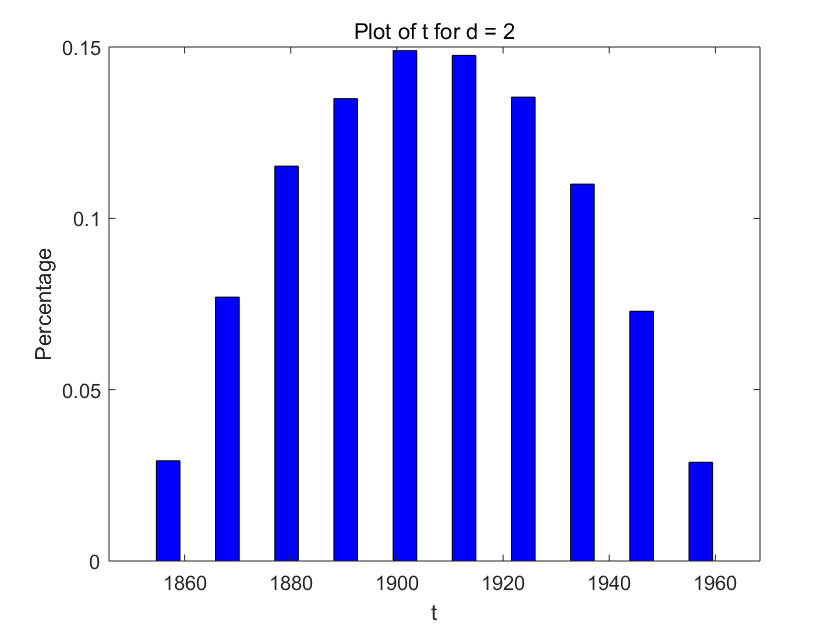
\includegraphics[width=130pt]{t_2.png}
    }
    \subfigure[$\lambda$]{
    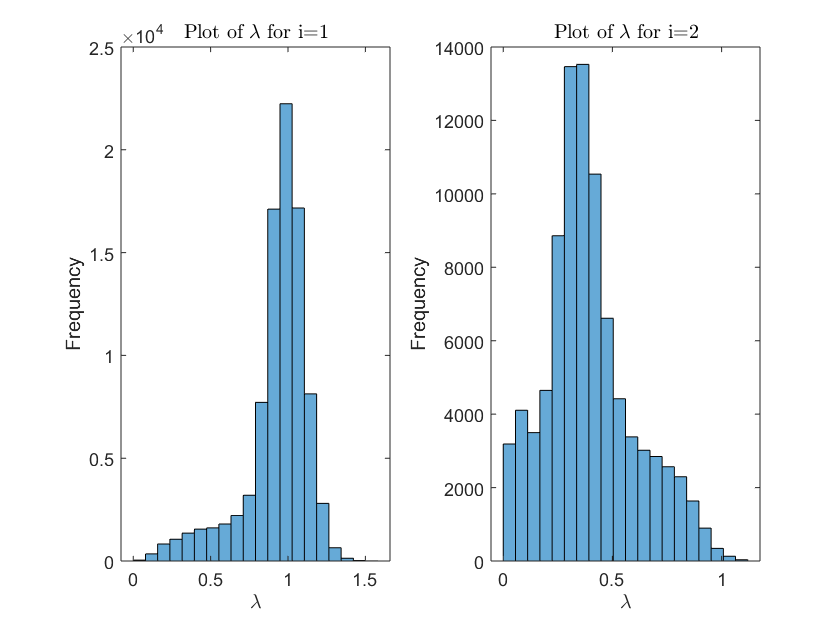
\includegraphics[width=130pt]{lambda_2.png}
    }
    \subfigure[$\theta$]{
    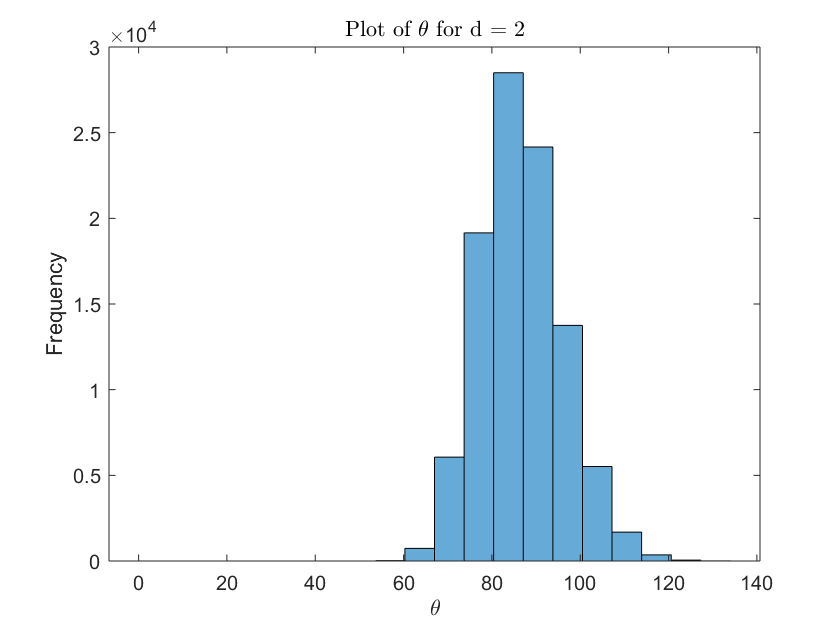
\includegraphics[width=130pt]{theta_2.png}
    }
    \caption{Break point=1}
\end{figure}

the histogram of t is centered around 1900, but the accuracy of estimation is not quite satisfying.

The histogram of $\lambda_1$ and $\lambda_2$ suggests that the intensities both have a $\Gamma$–distribution where the first intensity is centered around 1.1 whereas the second intensity is centered around 0.4, indicating a decrease of almost 70$\%$.

We can also see that $\theta$ intensity is centered around 90.

\subsubsection{two breakpoints}
\begin{figure}[H]
    \centering
    \subfigure[t]{
    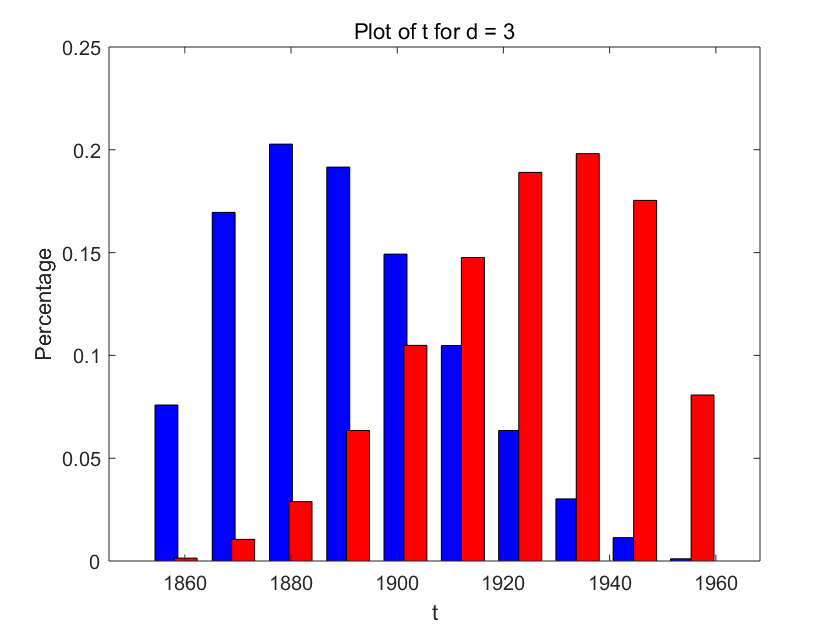
\includegraphics[width=130pt]{t_3.png}
    }
    \subfigure[$\lambda$]{
    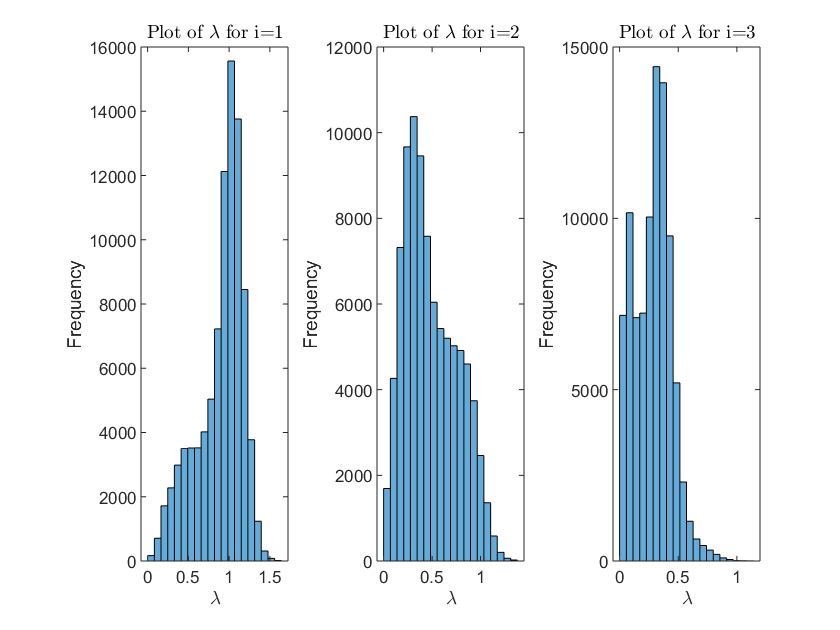
\includegraphics[width=130pt]{lambda_3.png}
    }
    \subfigure[$\theta$]{
    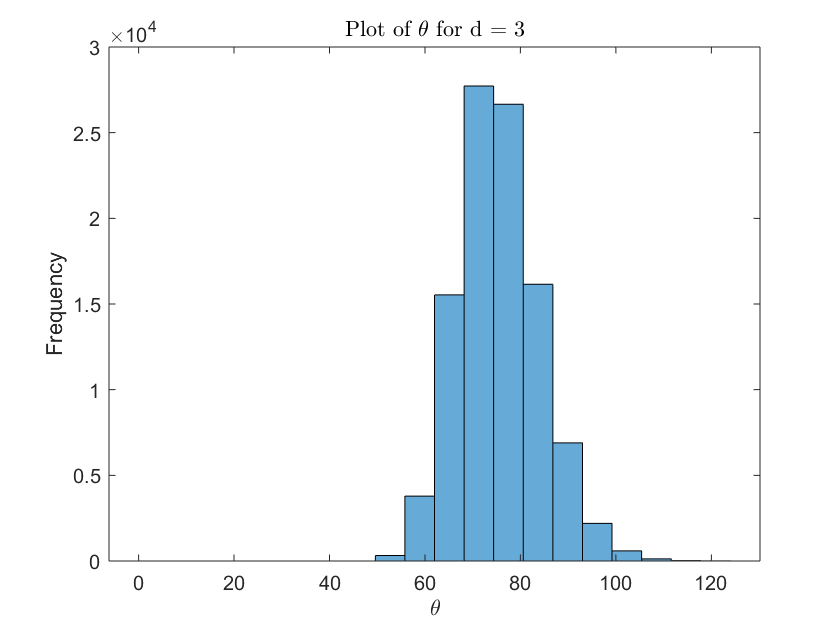
\includegraphics[width=130pt]{theta_3.png}
    }
    \caption{Break point=2}
\end{figure}

the histogram of t shows that the breakpoints are located at around 1890 and 1920.

The histogram of $\lambda_1$, $\lambda_2$ and $\lambda_3$ suggests that the intensities have a $\Gamma$–distribution and focus around 1.0, 0.4 and 0.3.

We can also see that $\theta$ intensity is centered around 80.


\subsubsection{three breakpoints}
\begin{figure}[H]
    \centering
    \subfigure[t]{
    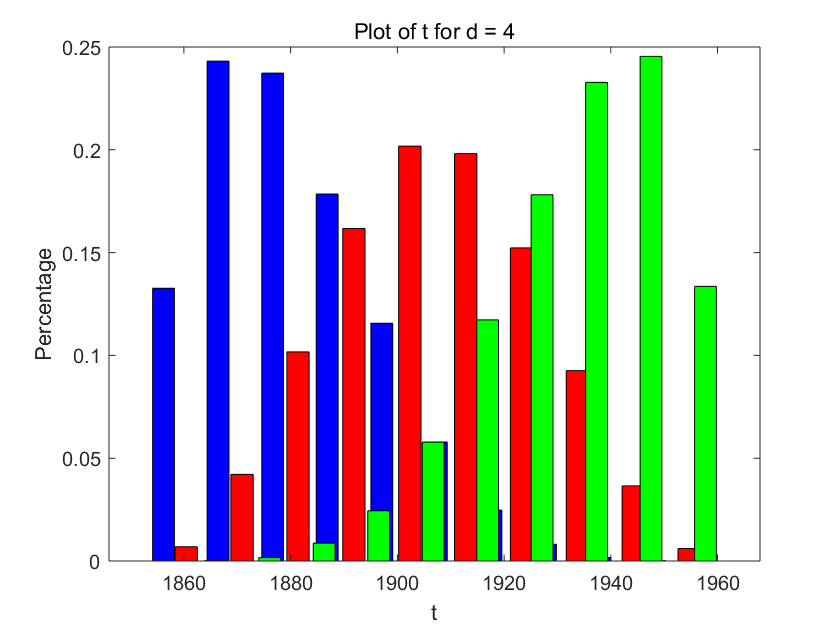
\includegraphics[width=130pt]{t_4.png}
    }
    \subfigure[$\lambda$]{
    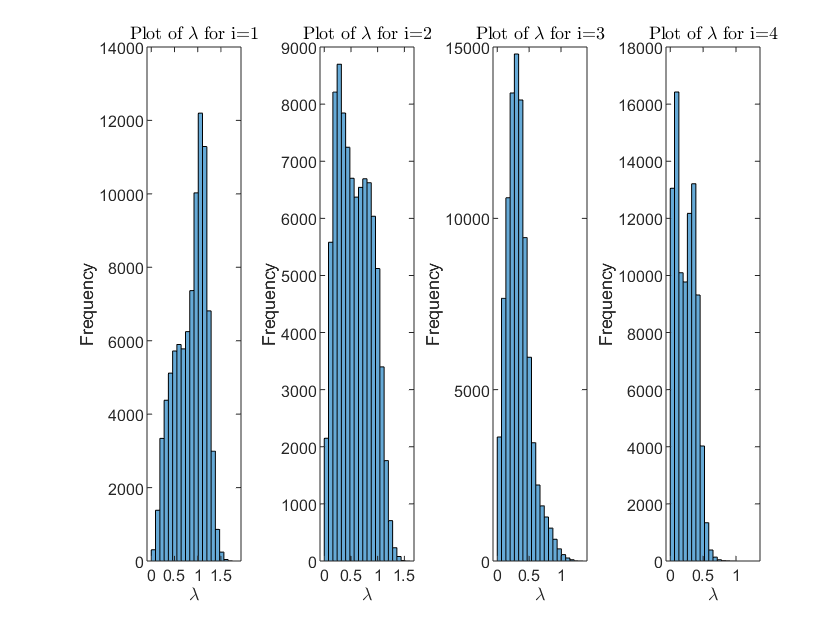
\includegraphics[width=130pt]{lambda_4.png}
    }
    \subfigure[$\theta$]{
    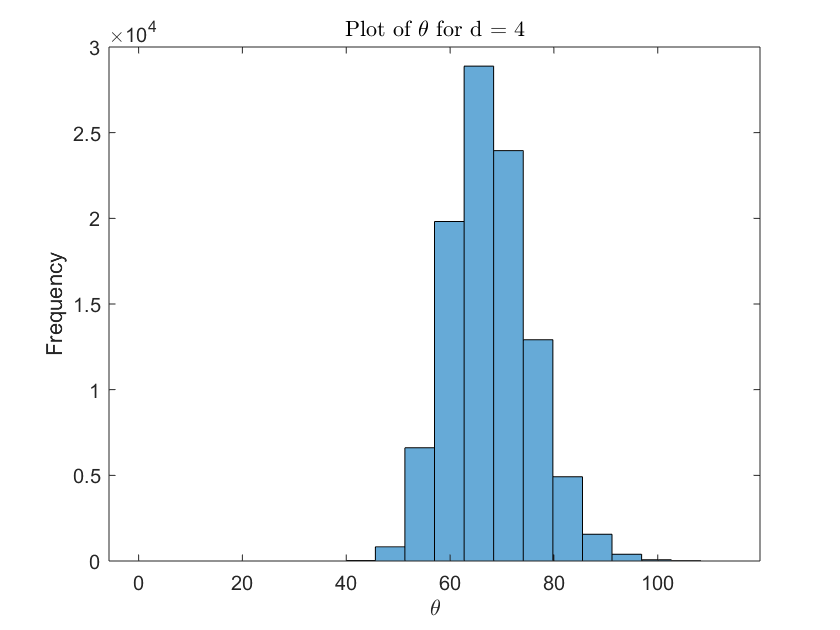
\includegraphics[width=130pt]{theta_4.png}
    }
    \caption{Break point=3}
\end{figure}

the histogram of t shows that the breakpoints are located at around 1880, 1910 and 1940. As we can easily distinguish the centers of densities in each breakpoint, the result is quite satisfying.

The histogram of $\boldsymbol{\lambda}$ suggests that the intensities have a $\Gamma$–distribution and focus around 1.0, 0.7,0.3 and 0.1.

We can also see that $\theta$ intensity is centered around 70.

\subsubsection{four breakpoints}
\begin{figure}[H]
    \centering
    \subfigure[t]{
    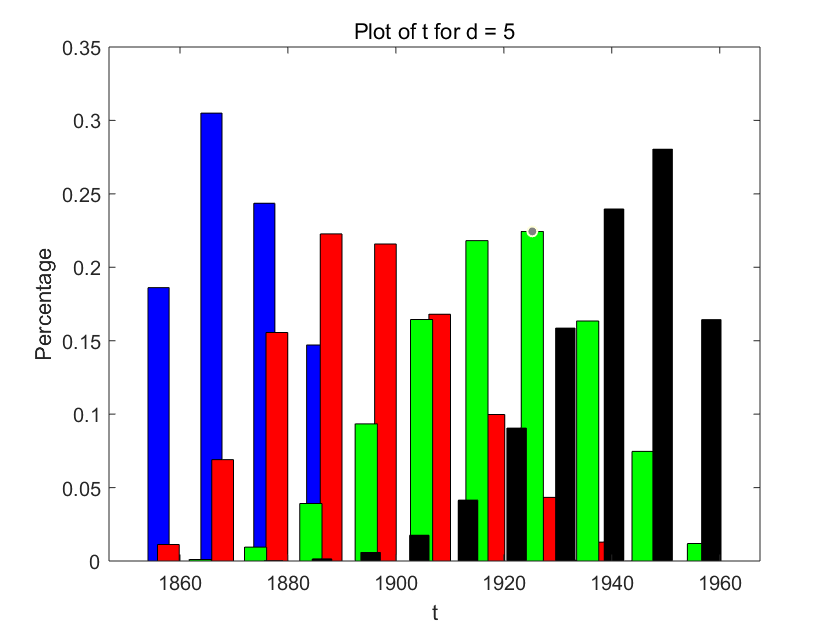
\includegraphics[width=130pt]{t_5.png}
    }
    \subfigure[$\lambda$]{
    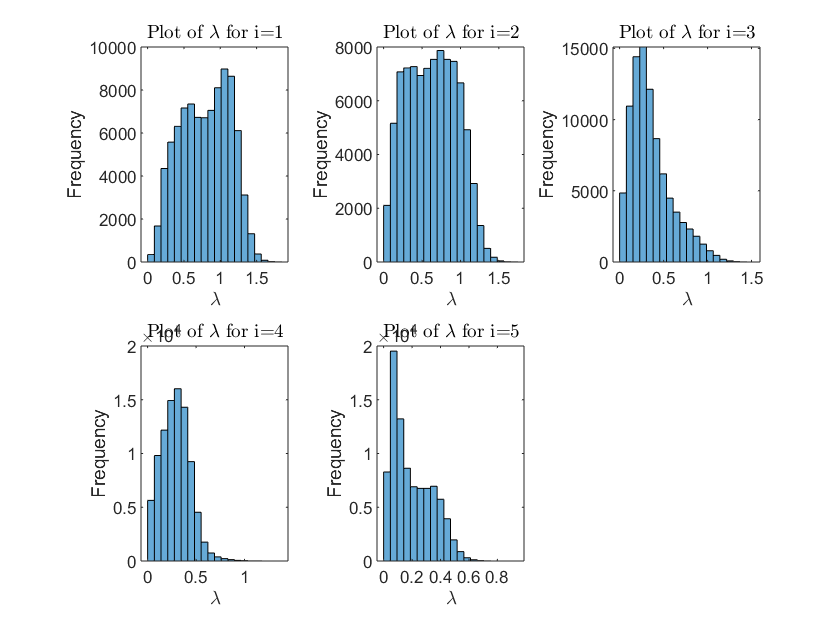
\includegraphics[width=130pt]{lambda_5.png}
    }
    \subfigure[$\theta$]{
    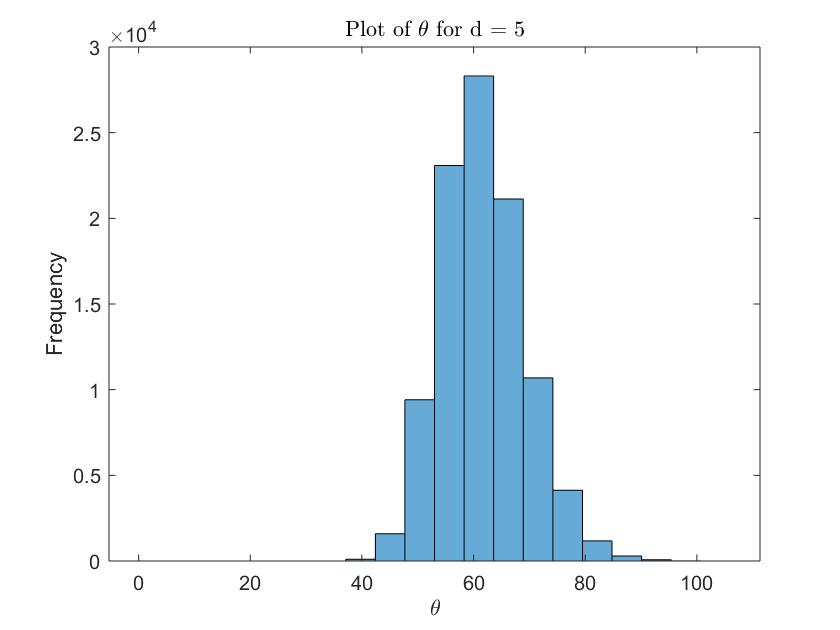
\includegraphics[width=130pt]{theta_5.png}
    }
    \caption{Break point=4}
\end{figure}

the histogram of t shows that the breakpoints are located at around 1870,1890,1920 and 1945. As we can easily distinguish the centers of densities in each breakpoint, the estimation is quite satisfying.

The histogram of $\boldsymbol{\lambda}$ suggests that the intensities have a $\Gamma$–distribution and focus around 1.0, 0.7, 0.25, 0.3 and 0.2.

We can also see that $\theta$ intensity is centered around 60.

\subsection{Sensitivity to the choice of $\vartheta$}
The sensitivity of the posteriors to the choice of $\vartheta$ is tested under the circumstance of 3 breakpoints and $\rho=1$.
\subsubsection{$\vartheta$ =1 }
\begin{figure}[H]
    \centering
    \subfigure[t]{
    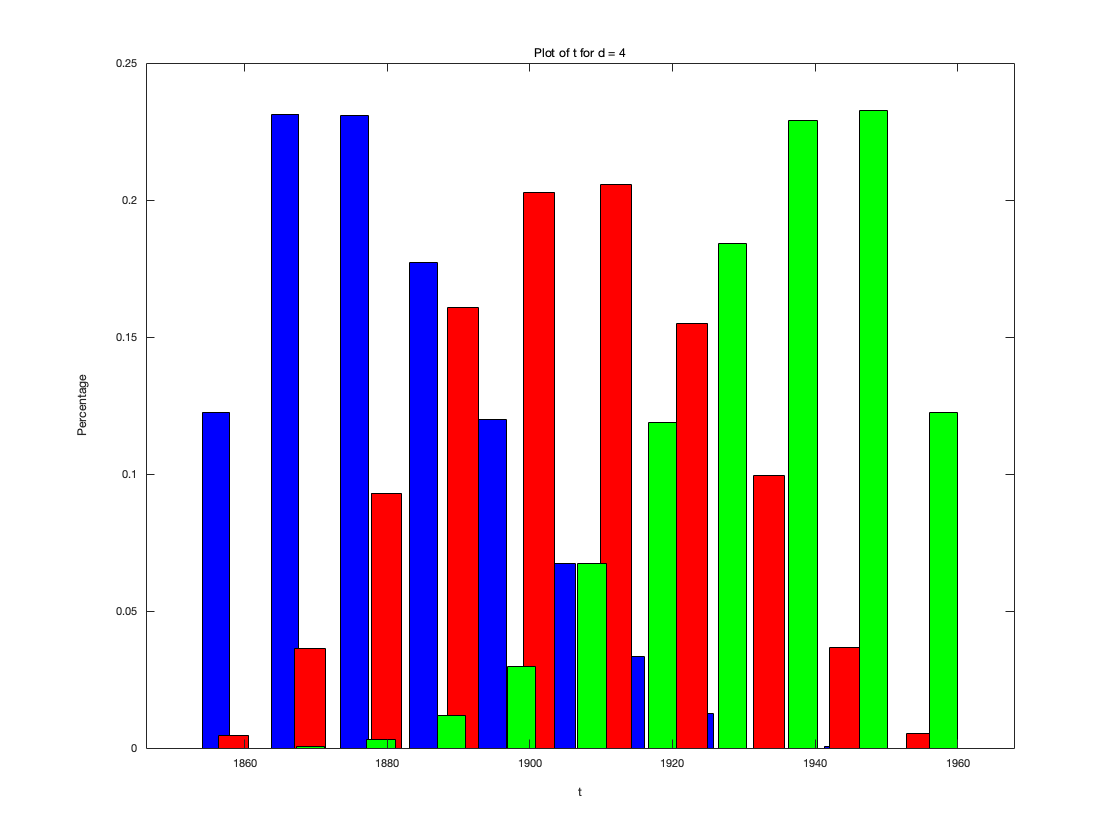
\includegraphics[width=130pt]{1-1.png}
    }
    \subfigure[$\lambda$]{
    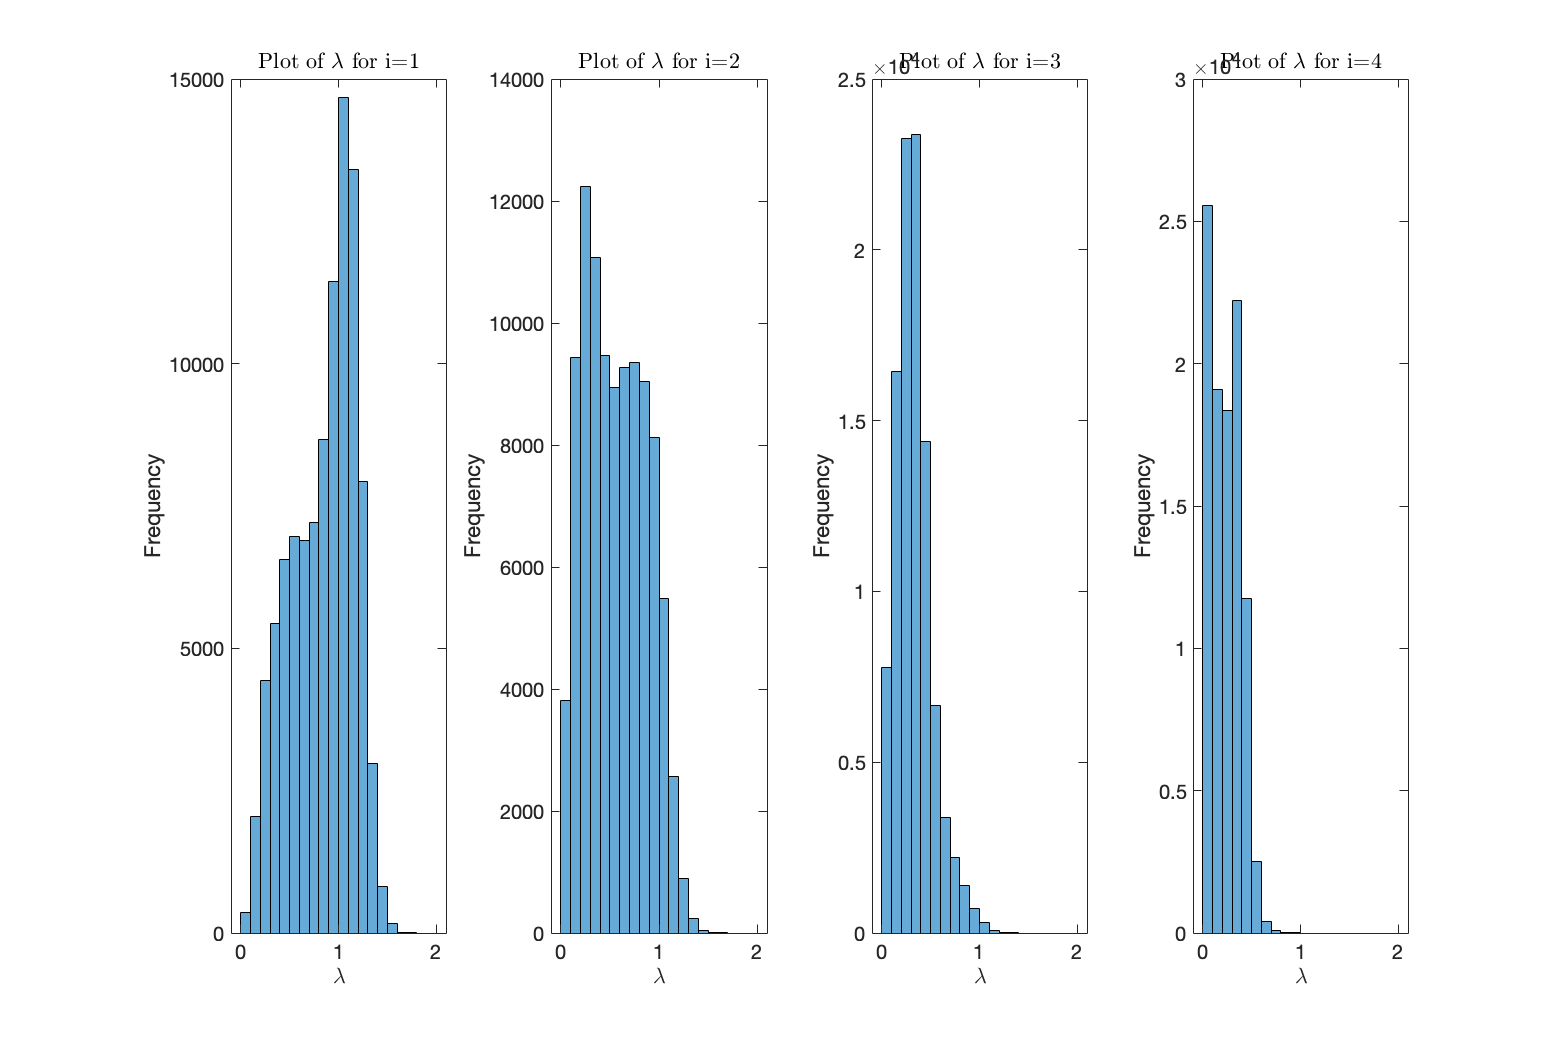
\includegraphics[width=130pt]{1-2.png}
    }
    \subfigure[$\theta$]{
    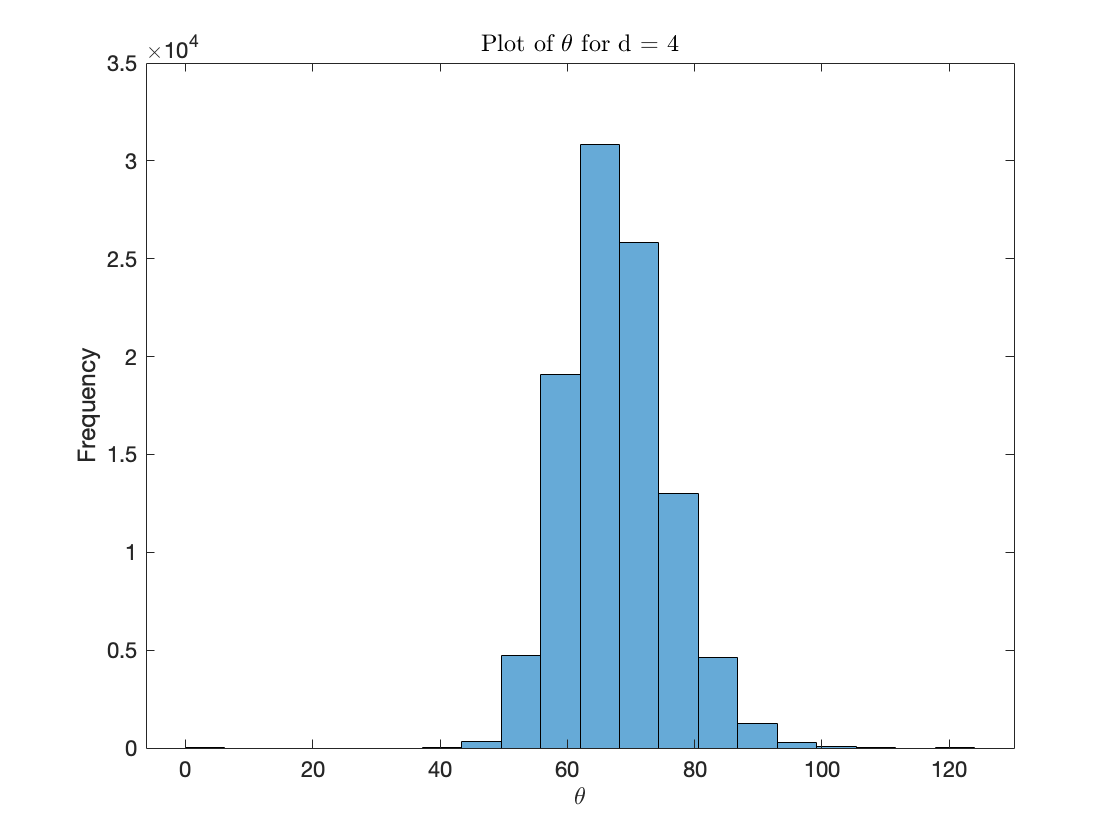
\includegraphics[width=130pt]{1-3.png}
    }
    \caption{$\vartheta$ =1}
\end{figure}

\subsubsection{$\vartheta$ =10 }
\begin{figure}[H]
    \centering
    \subfigure[t]{
    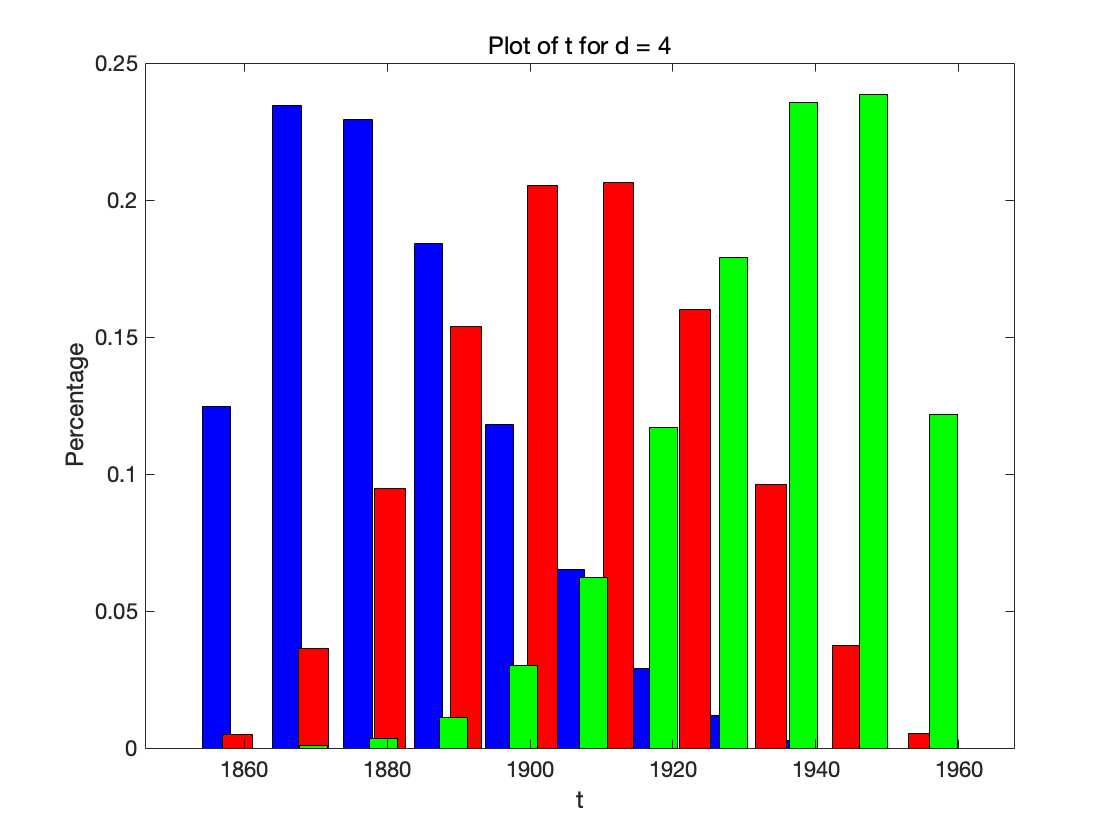
\includegraphics[width=130pt]{2-1.png}
    }
    \subfigure[$\lambda$]{
    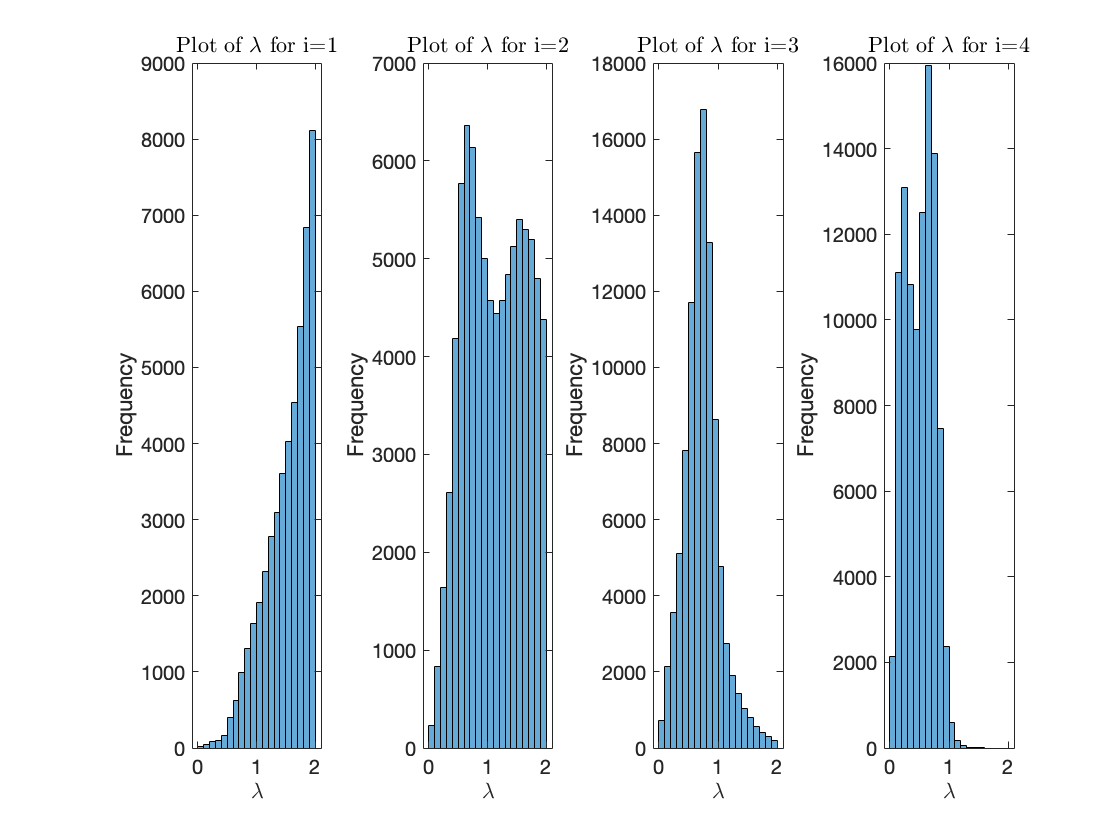
\includegraphics[width=130pt]{2-2.png}
    }
    \subfigure[$\theta$]{
    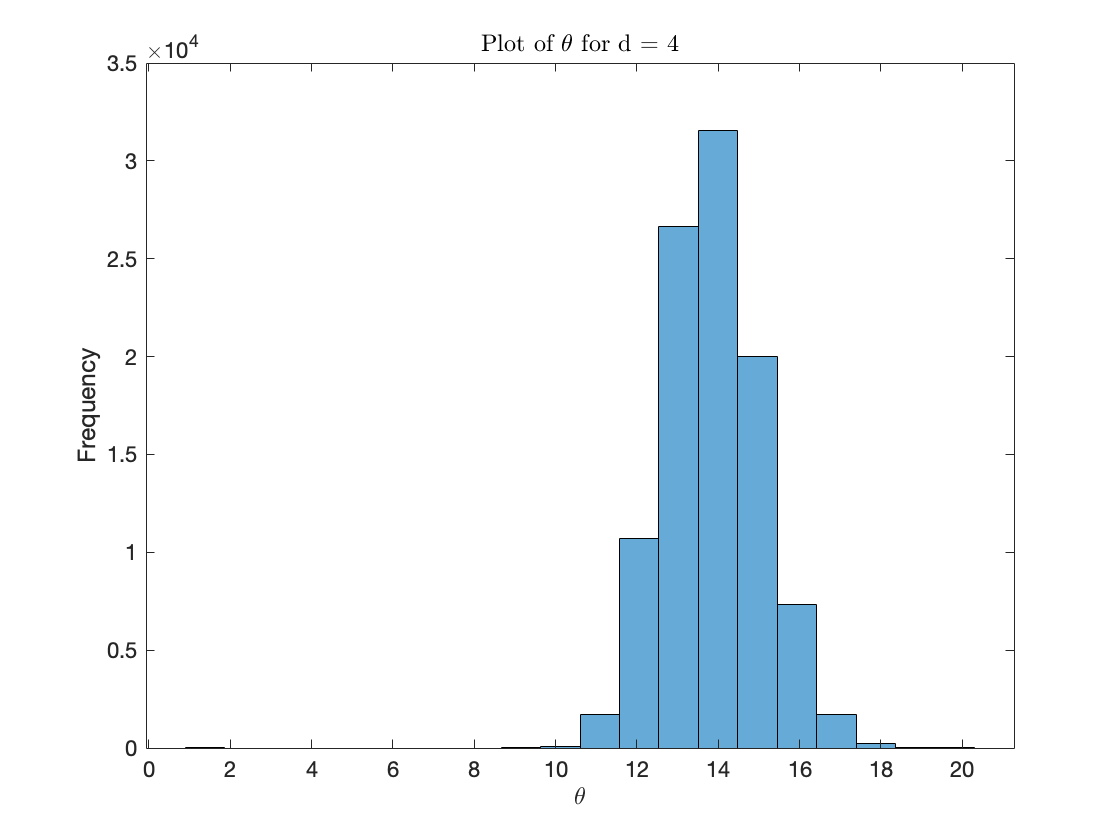
\includegraphics[width=130pt]{2-3.png}
    }
    \caption{$\vartheta$ =10}
\end{figure}

\subsubsection{$\vartheta$ =40 }
\begin{figure}[H]
    \centering
    \subfigure[t]{
    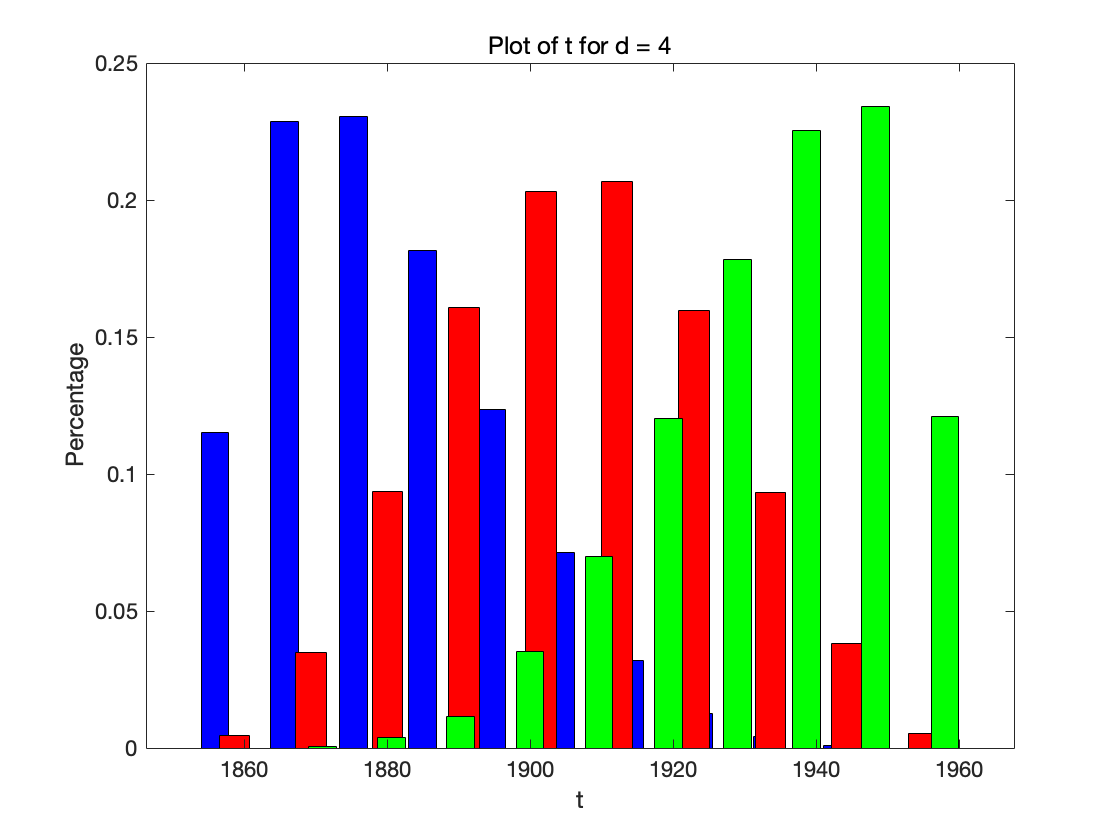
\includegraphics[width=130pt]{3-1.png}
    }
    \subfigure[$\lambda$]{
    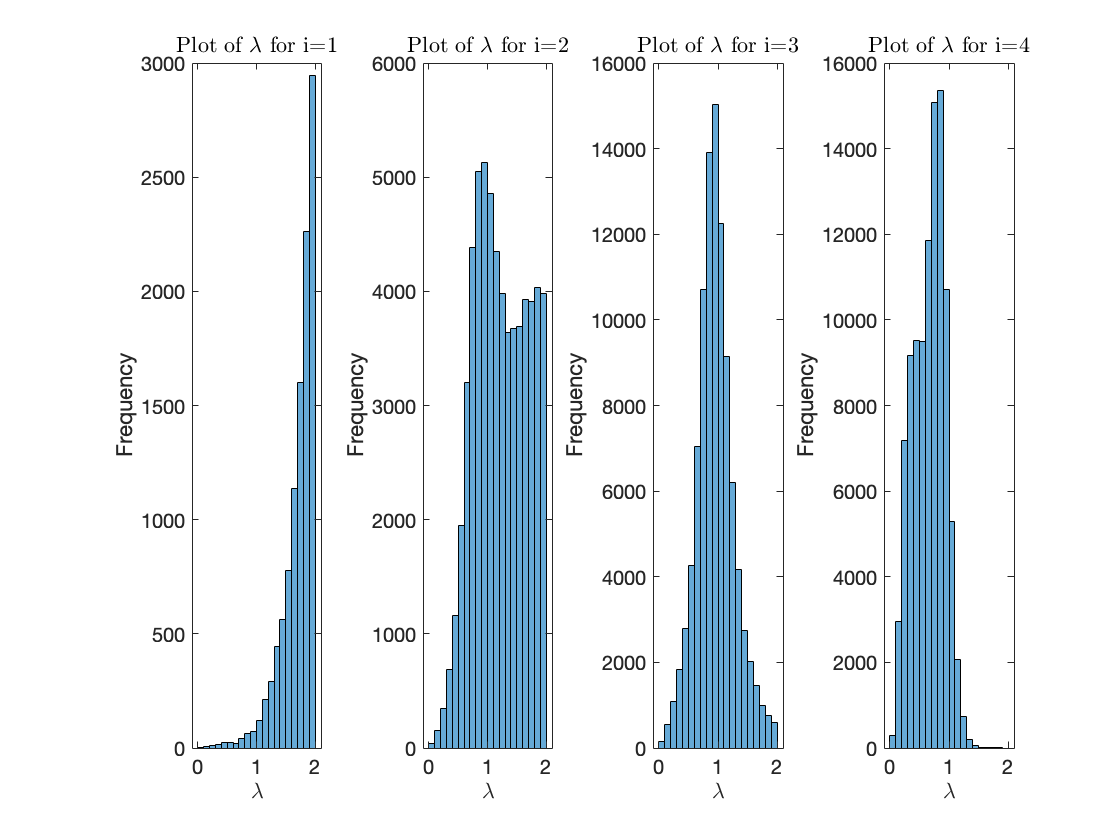
\includegraphics[width=130pt]{3-2.png}
    }
    \subfigure[$\theta$]{
    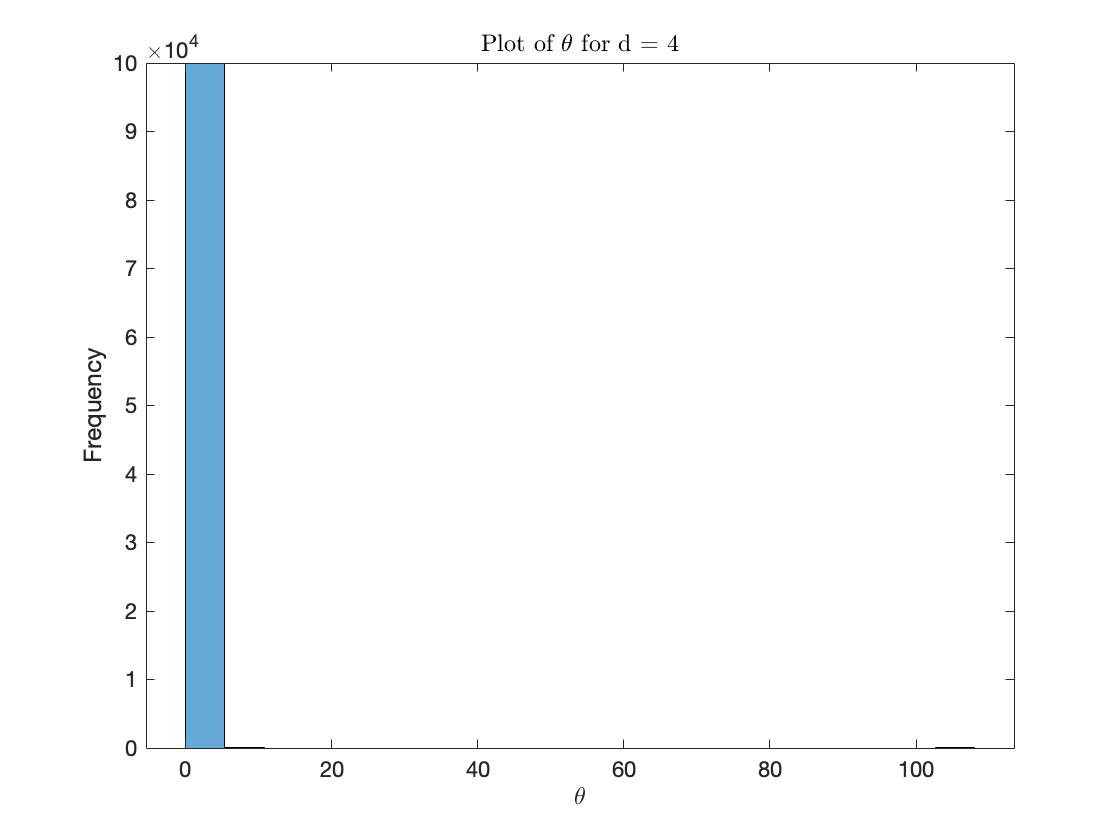
\includegraphics[width=130pt]{3-3.png}
    }
    \caption{$\vartheta$ =40}
\end{figure}

\subsubsection{$\vartheta$ =100 }
\begin{figure}[H]
    \centering
    \subfigure[t]{
    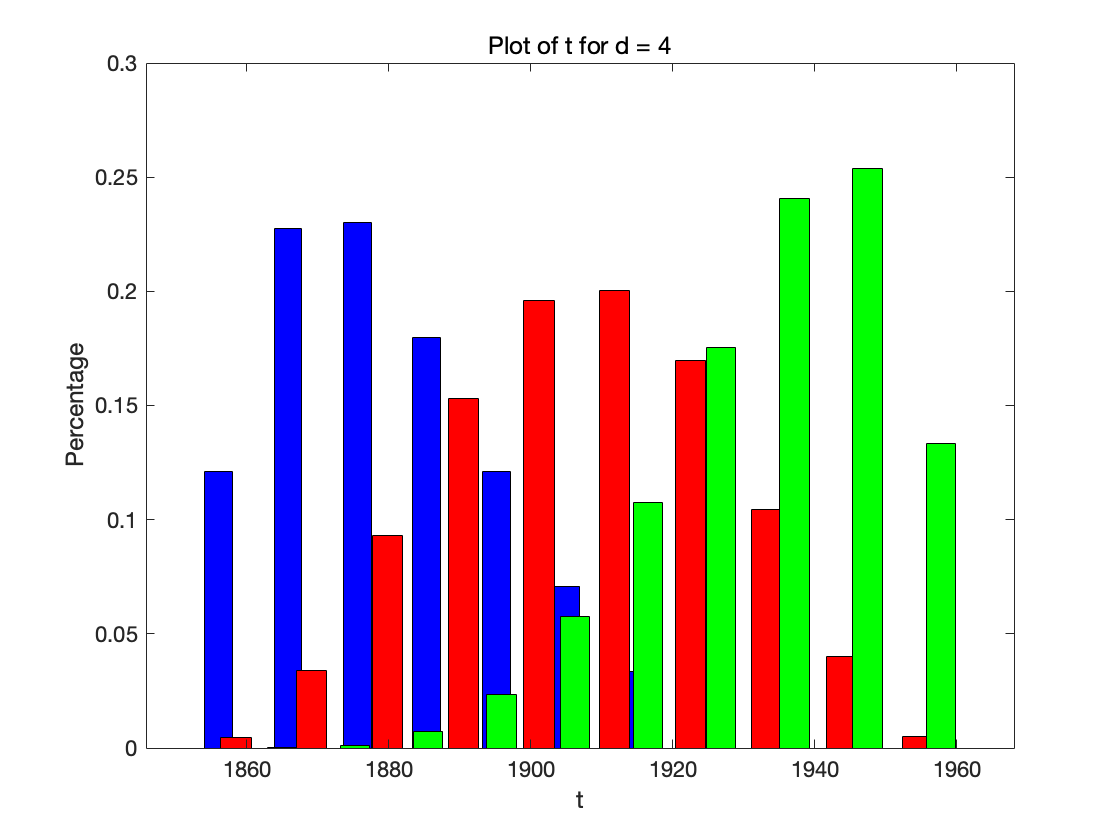
\includegraphics[width=130pt]{4-1.png}
    }
    \subfigure[$\lambda$]{
    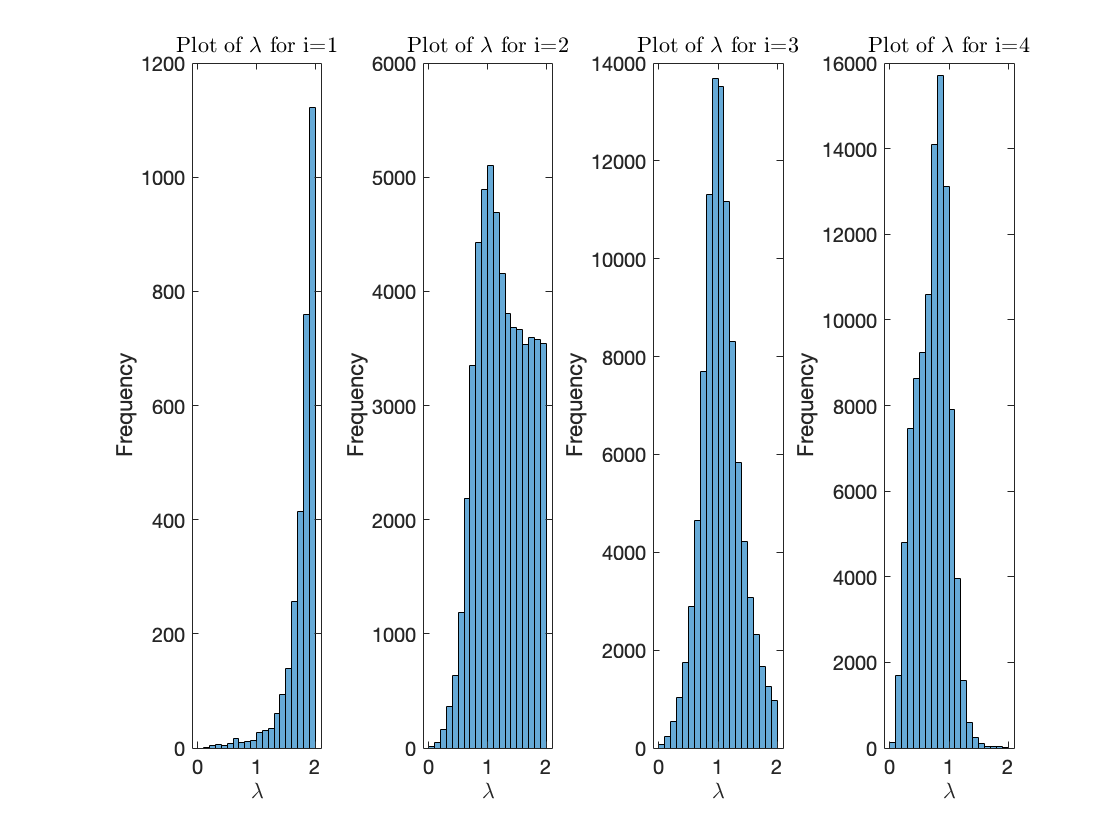
\includegraphics[width=130pt]{4-2.png}
    }
    \subfigure[$\theta$]{
    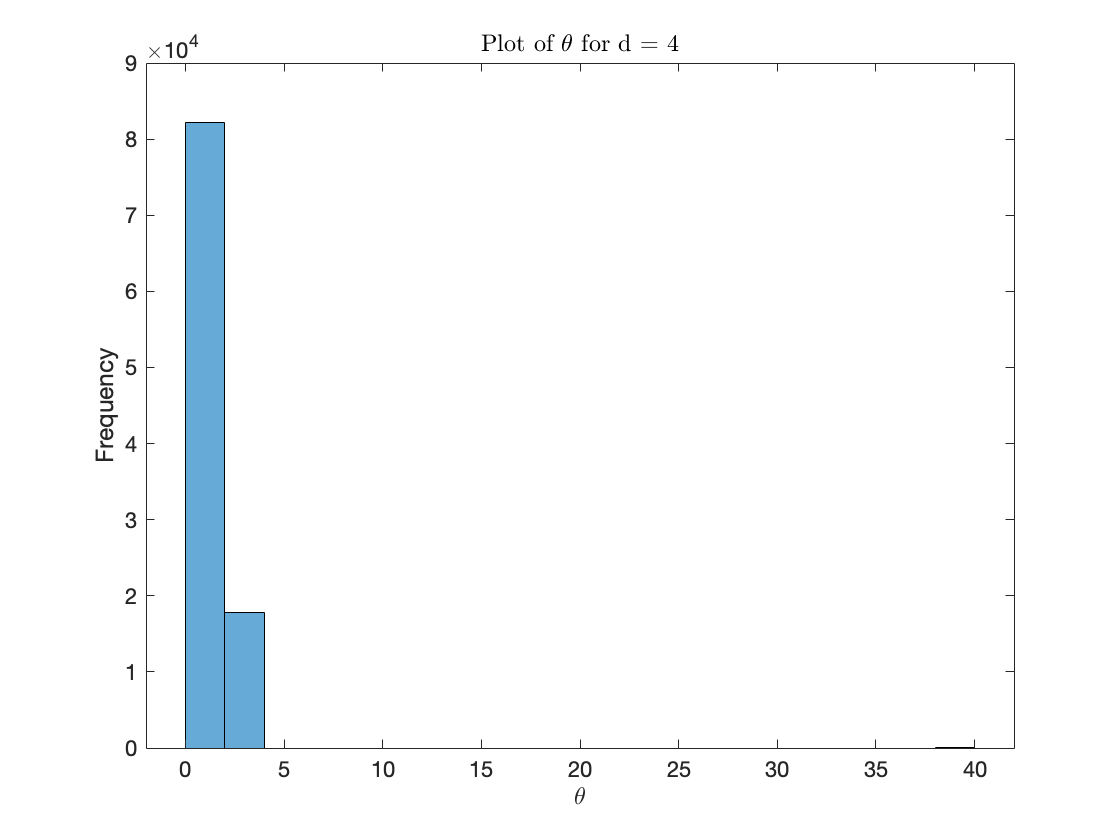
\includegraphics[width=130pt]{4-3.png}
    }
    \caption{$\vartheta$ =100}
\end{figure}

\subsubsection{Summary}

We estimated $t,\lambda,\theta$ with $\vartheta = 1,10,40,100$ and the conclusion is,
\begin{itemize}
    \item  $t$ is not sensitive to the choice of $\vartheta$
    \item $\lambda$ is not sensitive to $\vartheta$ within a centain range e.g. $[10,60]$. Even if $\vartheta$ was set to some extreme value e.g. $1$ or $100$, the estimated $\lambda$ just varies a bit.
    \item $\theta$ is quite sensitive to $\vartheta$, because the estimated $\theta$ tends to decrease when $\vartheta$ increases.
\end{itemize}

\subsection{Sensitivity to the choice of $\rho$}

The sensitivity of the posteriors to the choice of $\rho$ is tested under the circumstance of 3 breakpoints and $\vartheta=10$.
\subsubsection{$\rho$ =0.1 }
\begin{figure}[H]
    \centering
    \subfigure[t]{
    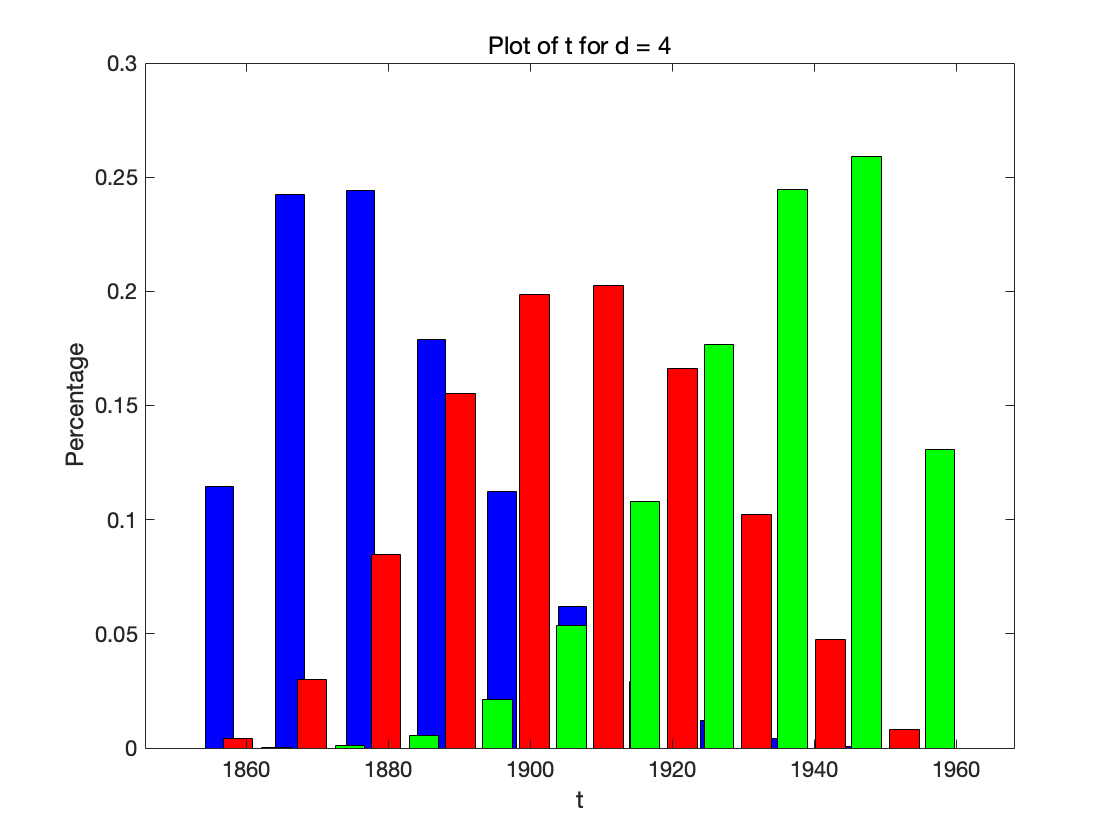
\includegraphics[width=130pt]{5-1.png}
    }
    \subfigure[$\lambda$]{
    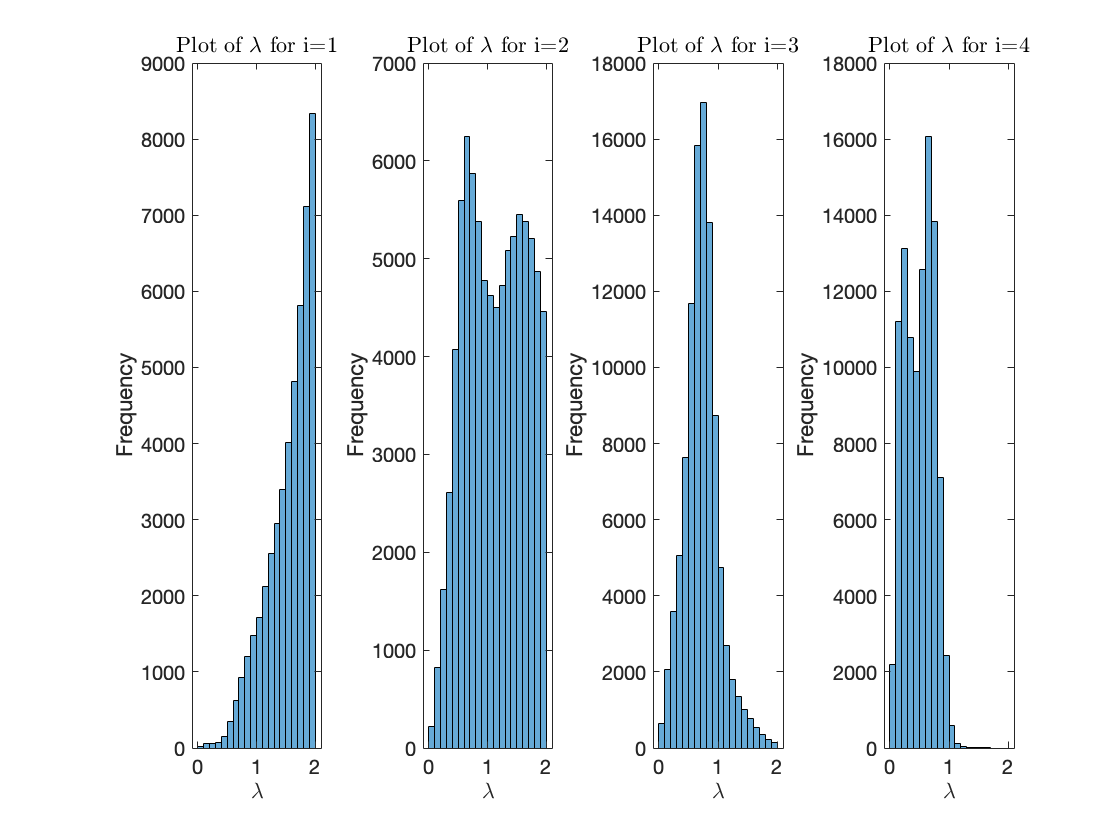
\includegraphics[width=130pt]{5-2.png}
    }
    \subfigure[$\theta$]{
    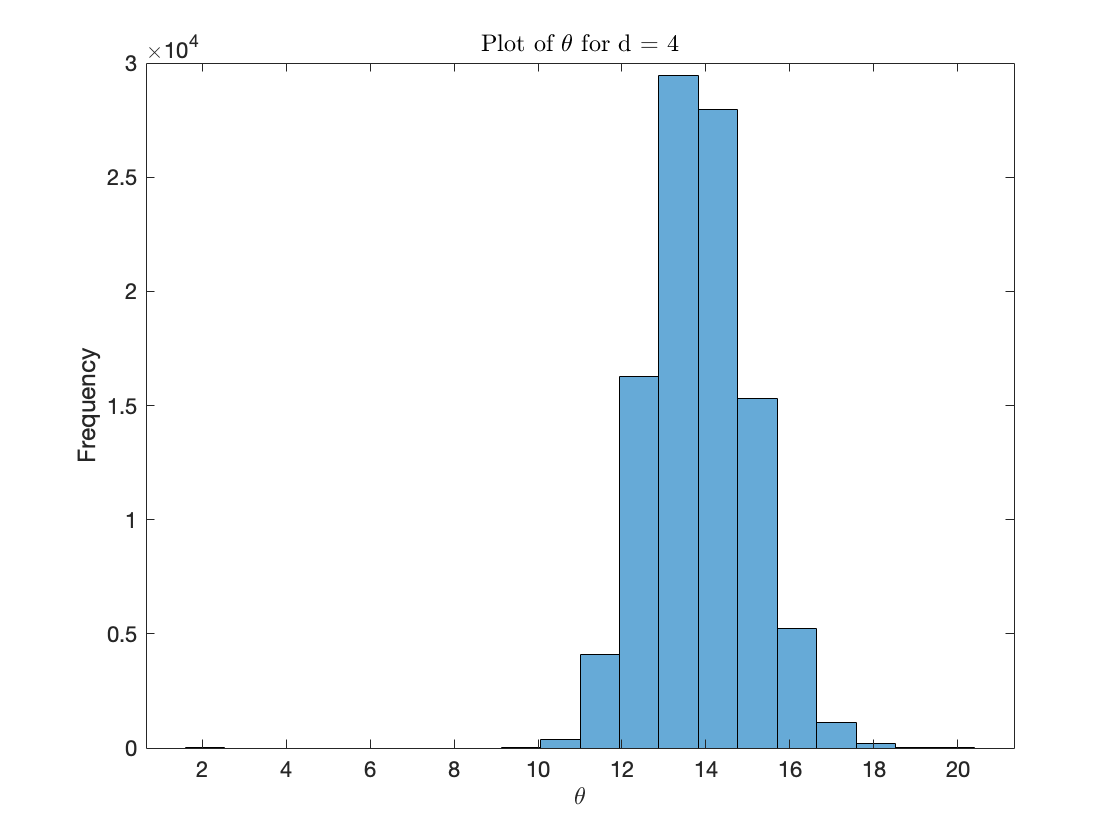
\includegraphics[width=130pt]{5-3.png}
    }
    \caption{$\rho$ =0.1}
\end{figure}

\subsubsection{$\rho$ =0.4 }
\begin{figure}[H]
    \centering
    \subfigure[t]{
    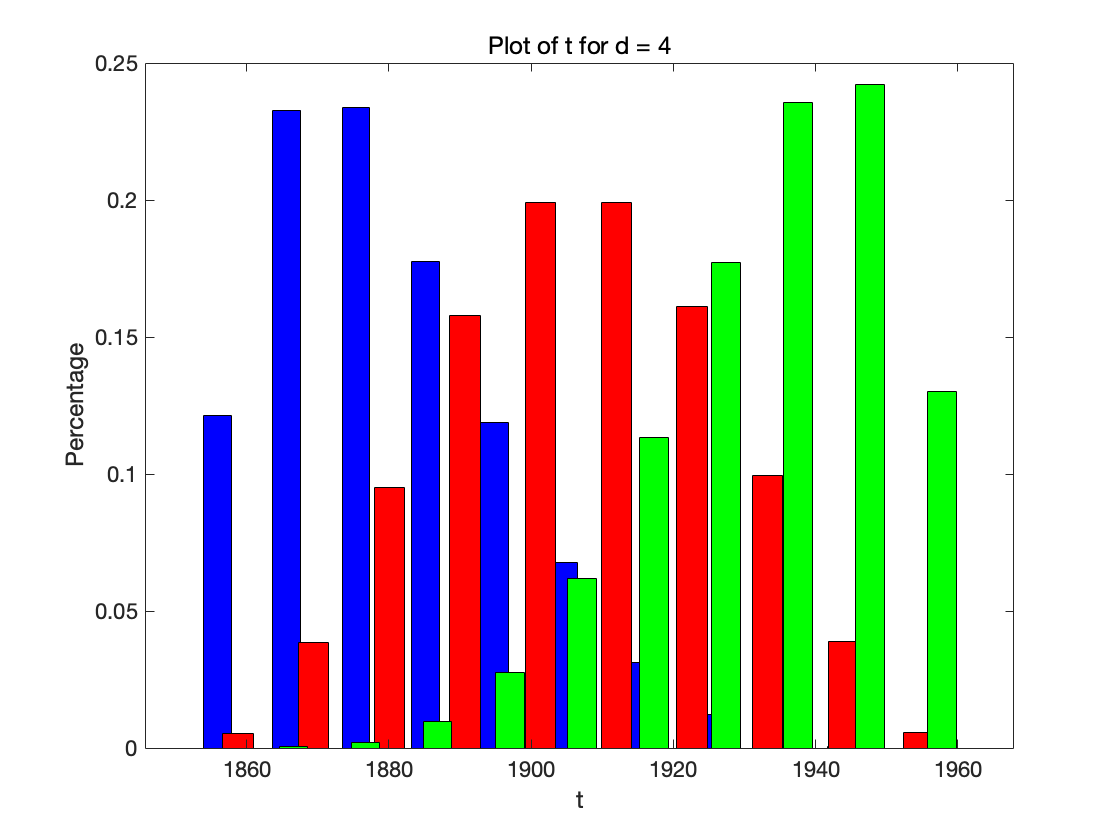
\includegraphics[width=130pt]{6-1.png}
    }
    \subfigure[$\lambda$]{
    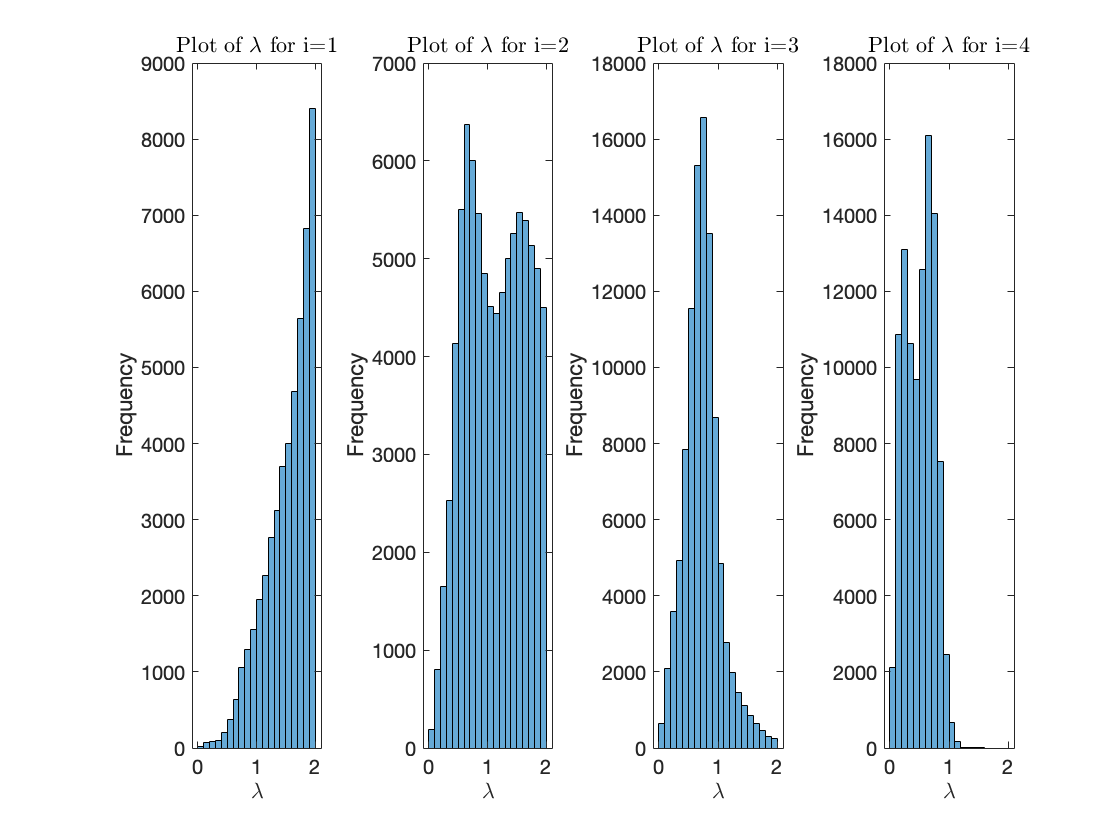
\includegraphics[width=130pt]{6-2.png}
    }
    \subfigure[$\theta$]{
    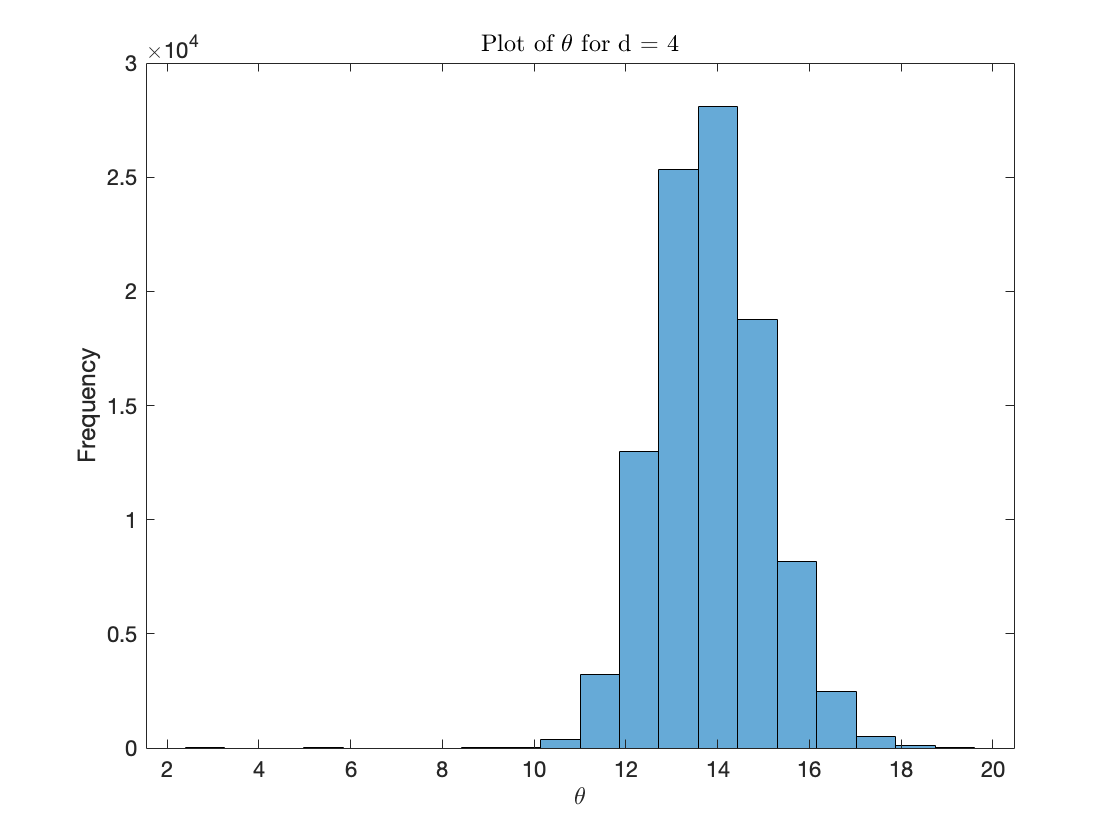
\includegraphics[width=130pt]{6-3.png}
    }
    \caption{$\rho$ =0.4}
\end{figure}

\subsubsection{$\rho$ =0.7 }
\begin{figure}[H]
    \centering
    \subfigure[t]{
    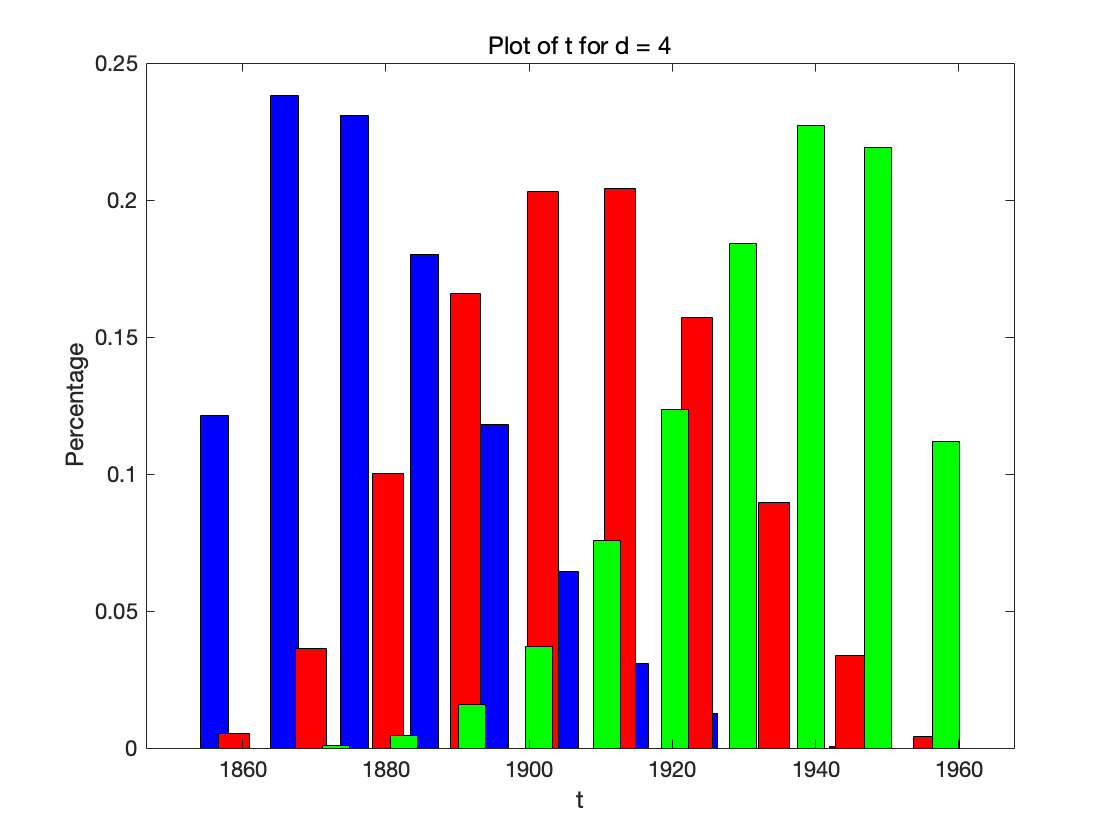
\includegraphics[width=130pt]{7-1.png}
    }
    \subfigure[$\lambda$]{
    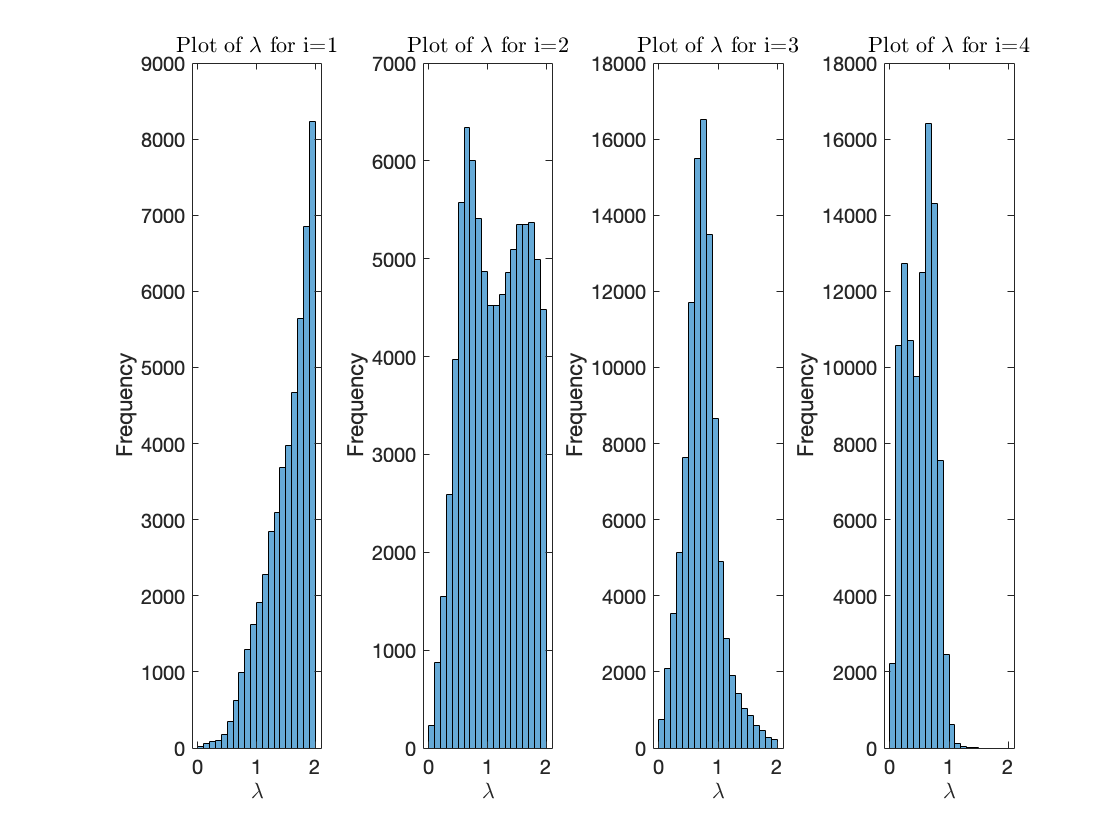
\includegraphics[width=130pt]{7-2.png}
    }
    \subfigure[$\theta$]{
    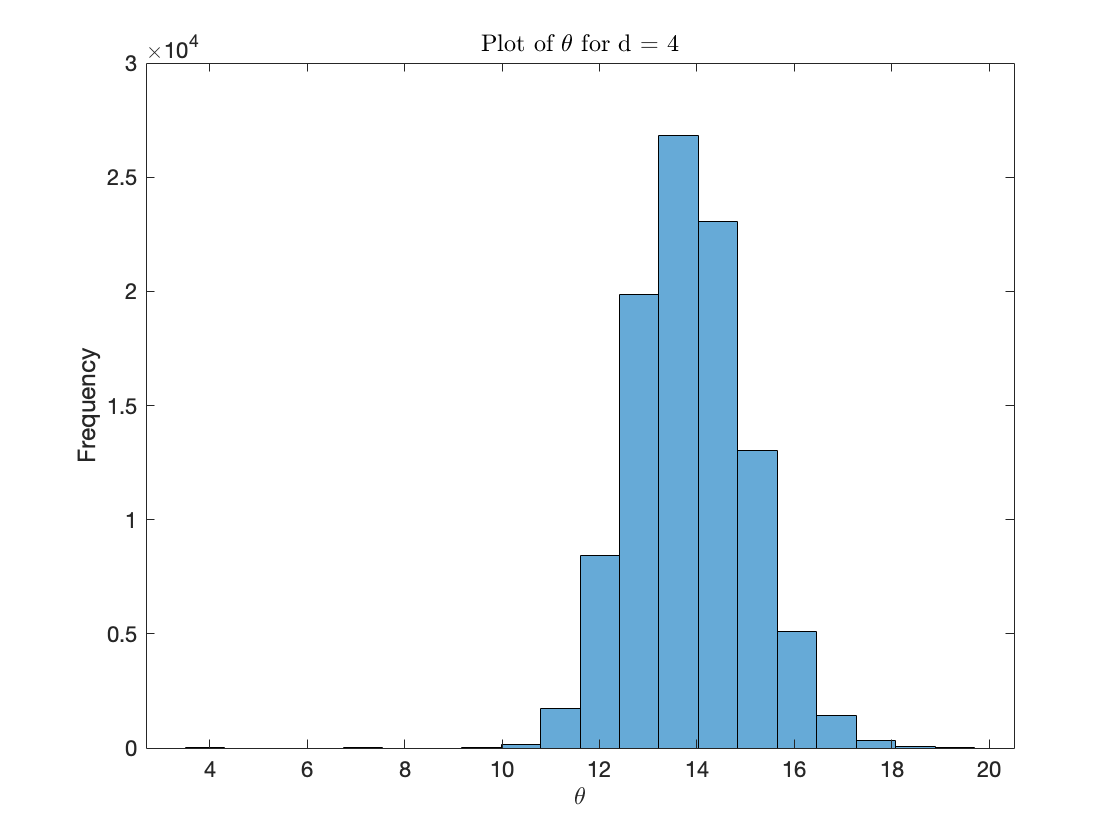
\includegraphics[width=130pt]{7-3.png}
    }
    \caption{$\rho$ =0.7}
\end{figure}

\subsubsection{$\rho$ =1.0 }
\begin{figure}[H]
    \centering
    \subfigure[t]{
    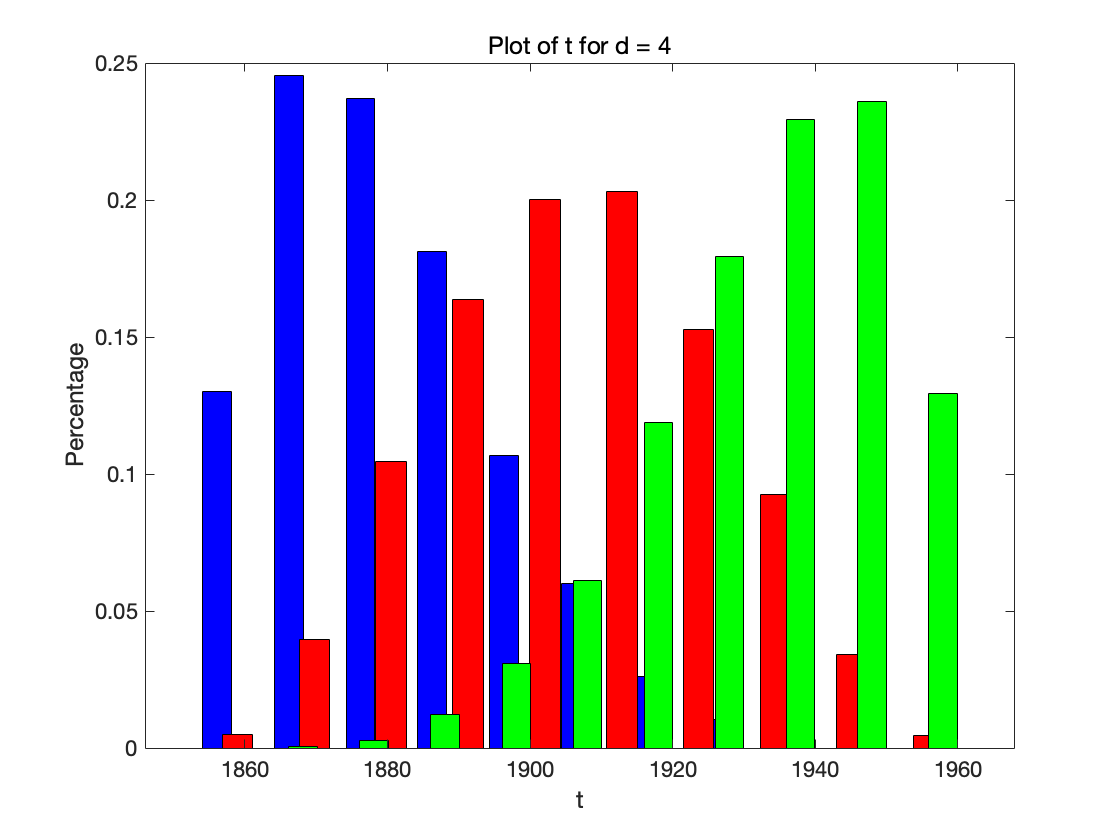
\includegraphics[width=130pt]{8-1.png}
    }
    \subfigure[$\lambda$]{
    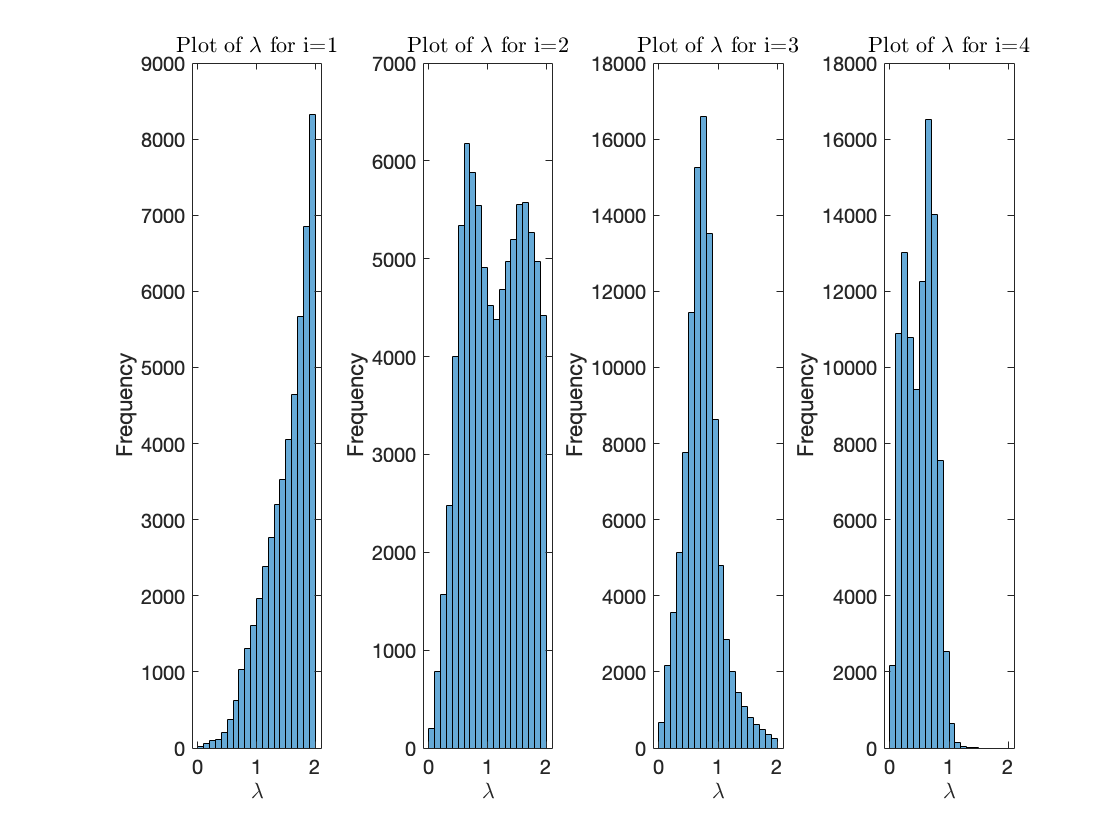
\includegraphics[width=130pt]{8-2.png}
    }
    \subfigure[$\theta$]{
    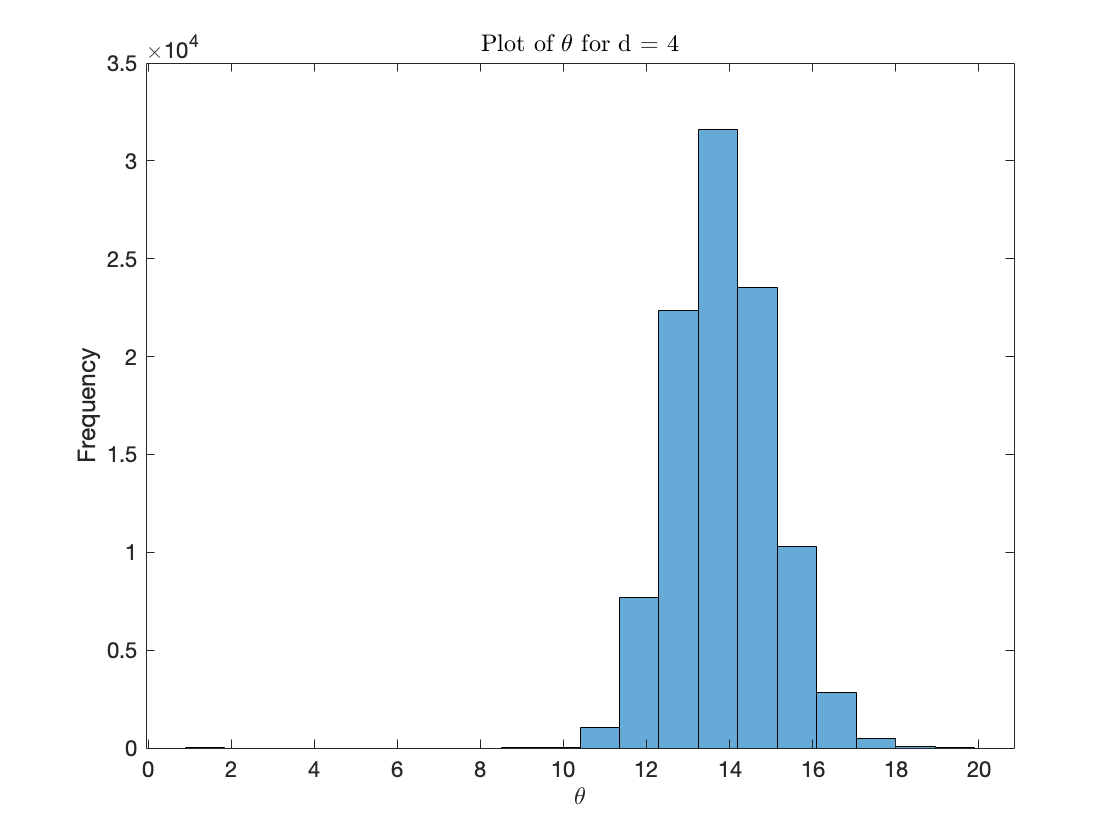
\includegraphics[width=130pt]{8-3.png}
    }
    \caption{$\rho$ =1.0}
\end{figure}

\subsubsection{Summary}

We estimated $t,\lambda,\theta$ with $\rho = 0.1,0.4,0.7,1.0$ and the conclusion is all the posteriors are not sensitive to the choice of $\rho$.

Also, from the figures of t-posteriors, we can conclude that the mixing for t is also not sensitive to the choice of $\rho$.

\section{EM-based inference in mixture models}
\subsection{complete data log-likelihood function $f_\theta(\boldsymbol{x},\boldsymbol{y})$}
\begin{equation*}
\begin{split}
    f_\theta(\boldsymbol{x},\boldsymbol{y}) = \prod_{i=1}^n f_\theta(x_i,y_i) 
\end{split}
\end{equation*}
where 
\begin{equation*}
        f_\theta(x_i,y_i)=f_\theta(y_i|x_i=0)p_\theta(x_i=0)(1-x_i)+f_\theta(y_i|x_i=1)p_\theta(x_i=1)x_i 
        \\= g_0(y_i)(1-\theta)(1-x_i)+g_1(y_i)\theta x_i
\end{equation*}


Thus, 

\begin{equation*}
    \log f_\theta(\boldsymbol{x},\boldsymbol{y})=\sum_{i=1}^n \log [g_0(y_i)(1-\theta)(1-x_i)+g_1(y_i)\theta x_i]
\end{equation*}

\subsection{conditional distribution $f_\theta(\boldsymbol{x}|\boldsymbol{y})$}

\begin{equation*}
        f_\theta(\boldsymbol{x}|\boldsymbol{y}) &= \frac{f_\theta(\boldsymbol{x},\boldsymbol{y})}{f_\theta(\boldsymbol{y})} 
\end{equation*}

Since 
\begin{equation*}
        f_\theta(y_i) =  f_\theta(x_i=1,y_i)p_\theta (x_i=1)+ f_\theta(x_i=0,y_i)p_\theta (x_i=0)
        \\=g_0(y_i)(1-\theta)+ g_1(y_i)\theta
\end{equation*}


Thus, $X_i | Y_i $ is a Bernoulli distribution, where $P(X_i=1 | Y_i)=\frac{g_1(y_i)\theta}{g_0(y_i)(1-\theta)+ g_1(y_i)\theta}$
\begin{equation}
    f_\theta(\boldsymbol{x}|\boldsymbol{y})=\frac{\prod_{i=1}^n[g_0(y_i)(1-\theta)(1-x_i)+g_1(y_i)\theta x_i]}{\prod_{i=1}^n (g_0(y_i)(1-\theta)+ g_1(y_i)\theta)}
\end{equation}


\subsection{EM algorithm for $\theta$}
The data is inspected by plotting a histogram.
\begin{figure}[H]
    \center{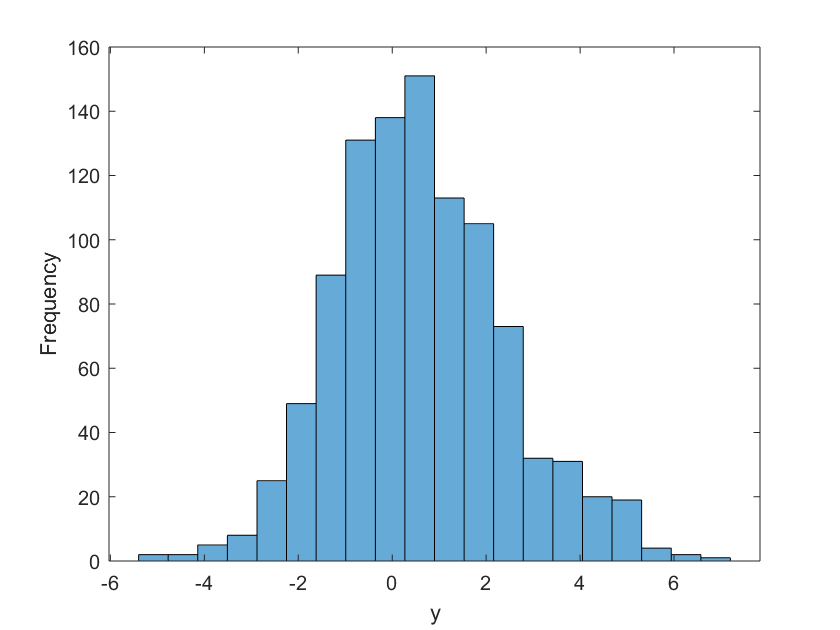
\includegraphics[width=230pt]{EM_1.png}}
\end{figure}

In the E- step, 
\begin{equation*}
    \centering
    \begin{aligned}
     Q_{\theta_l}(\theta)=\mathbb{E}_{\theta_l}(\log f_\theta(\textbf{X},\textbf{Y})|\textbf{Y})&=\mathbb{E}_{\theta_l}(\sum_{i=1}^n \log f_{\theta}(x_i,y_i)|y_i)  
     \\
     & =\mathbb{E}_{\theta_l}(\sum_{i=1}^n \log [g_0(y_i)(1-\theta)(1-x_i)+g_1(y_i)\theta x_i])
     \\
     &=\sum_{i=1}^n \left[\log(g_0(y_i)(1-\theta))\right P_{\theta_l} (x_i=0 | y_i)+\log(g_1(y_i)\theta)\right P_{\theta_l} (x_i=1 | y_i)]
     \\
     &= \sum_{i=1}^n\left[\frac{g_0(y_i)(1-\theta_l)\log(1-\theta)+g_1(y_i)\theta_l log(\theta)}{g_0(y_i)(1-\theta_l)+g_1(y_i)\theta_l)}\right]+ \text{constant} 
    \end{aligned}
    
\end{equation*}
Denote $p_{i}= \frac{g_1(y_i)\theta_l}{g_0(y_i)(1-\theta_l)+g_1(y_i)\theta_l)}$, so $Q_{\theta_l}(\theta)=\sum_{i=1}^n ((1-p_{i})log(1-\theta)+p_{i}log(\theta))$

In the M-step


\begin{equation*}
    \begin{align*}
       Q_{\theta_l}'(\theta)=0\Longrightarrow \frac{\sum_{i=1}^n p_i}{\theta} = \frac{\sum_{i=1}^n (1-p_i) }{1-\theta}
    \\
    \theta_{l+1}=\operatorname{argmax} \mathscr{Q}(\theta)=\frac{1}{N} \sum_{i=1}^{N} \frac{\theta_l g_1(y_i)}{\theta_l g_1(y_i)+ (1-\theta_l) g_0(y_i)} 
    \end{align*}
    
\end{equation*}
\begin{figure}[H]
    \center{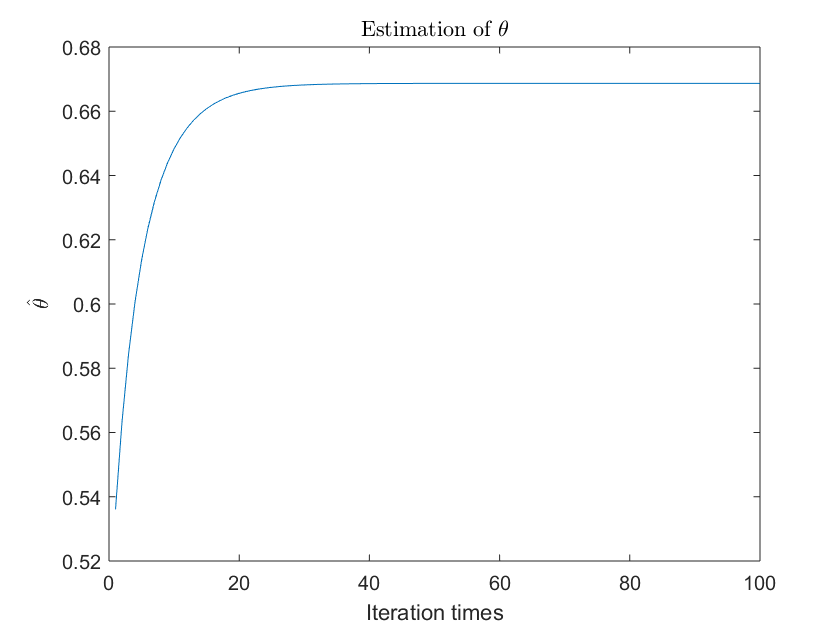
\includegraphics[width=230pt]{EM_2.png}}
\end{figure}

We set the initial $\theta_0$ to 0.5. As shown in the figure above, the final estimator is 0.66868.

\end{document}
